\clearpage
\renewcommand{\thesection}{\Alph{section}}
\setcounter{section}{0}

\begin{center}
    \textbf{\Large ~\ours: Large-Scale Driving Scene Generation with \\[0.4em] High Fidelity and Flexible Controllability}\\[1.2em]
    \large Supplementary Material
\end{center}

\vspace{1.2em}
{\large \textbf{Contents}}

\startcontents[appendices]
\printcontents[appendices]{l}{1}{\setcounter{tocdepth}{3}}

\clearpage
\section{Additional Implementation Details}
In this section, we provide additional implementation details to facilitate reproducibility. Specifically, we elaborate on the experimental datasets, model implementation, and the evaluation metrics.


\subsection{Datasets}
We use Occ3D-nuScenes~\cite{Occ3D} to train our controllable occupancy generation module, and nuScenes~\cite{nuScenes} for the multi-view image and video generation modules. The textual scene graph-to-layout generation module is also trained using 3D bounding box and HD map annotations from nuScenes. The dataset comprises 1,000 driving scenes under diverse weather, lighting, and traffic conditions. Each 20-second scene includes about 40 annotated keyframes, yielding roughly 40,000 samples with 360° multi-view images, 3D occupancy, bounding boxes, and maps. We follow the standard split of 700 training and 150 validation scenes. For video generation, ASAP interpolation is applied to upsample the frame rate from 2 Hz to 12 Hz, yielding about 240 frames per scene and enabling more consistent training for temporally coherent video synthesis.
Following DynamicCity~\cite{DynamicCity}, we map the original 17 semantic categories to 11 commonly used classes (see Table~\ref{tab:supp_mapping}) and conduct experiments both with and without label mapping to enable comprehensive comparisons.

\definecolor{building}{RGB}{222, 184, 135}
\definecolor{barrier}{RGB}{112, 128, 144}
\definecolor{free}{RGB}{240, 240, 240}
\definecolor{pedestrian}{RGB}{0, 0, 255}
\definecolor{pole}{RGB}{153, 153, 153}
\definecolor{road}{RGB}{217, 217, 217}
\definecolor{ground}{RGB}{23, 135, 31}
\definecolor{sidewalk}{RGB}{255, 52, 179}
\definecolor{vegetation}{RGB}{84, 255, 159}
\definecolor{vehicle}{RGB}{255, 158, 0}
\definecolor{bicycle}{RGB}{220, 20, 60}

\begin{table}[ht]
    \centering
    \scriptsize
    \setlength{\tabcolsep}{1pt}
    \renewcommand{\arraystretch}{0.8}
    \caption{\textbf{Summary of Semantic Label Mappings}. We map the original 17-class nuScenes semantic labels to 11 classes following the protocol in~\cite{DynamicCity} to enable comprehensive evaluation.}
    \resizebox{\linewidth}{!}{%
    \begin{tabular}{@{}c|*{11}{>{\centering\arraybackslash}m{1.1cm}@{}}}
    \toprule
    \makecell[t]{\textbf{Mapped} \\ \textbf{Class} \\ 11} & 
    \rotatebox{60}{\textcolor{building}{$\blacksquare$} Building} & 
    \rotatebox{60}{\textcolor{barrier}{$\blacksquare$} Barrier} & 
    \rotatebox{60}{\textcolor{free}{$\blacksquare$} Free} & 
    \rotatebox{60}{\textcolor{pedestrian}{$\blacksquare$} Pedestrian} & 
    \rotatebox{60}{\textcolor{pole}{$\blacksquare$} Pole} & 
    \rotatebox{60}{\textcolor{road}{$\blacksquare$} Road} & 
    \rotatebox{60}{\textcolor{ground}{$\blacksquare$} Ground} & 
    \rotatebox{60}{\textcolor{sidewalk}{$\blacksquare$} Sidewalk} & 
    \rotatebox{60}{\textcolor{vegetation}{$\blacksquare$} Vegetation} & 
    \rotatebox{60}{\textcolor{vehicle}{$\blacksquare$} Vehicle} & 
    \rotatebox{60}{\textcolor{bicycle}{$\blacksquare$} Bicycle} \\
    \midrule
    \makecell[t]{\textbf{Original} \\ \textbf{Class} \\ 17} & 
    \rotatebox{60}{Manmade} & 
    \rotatebox{60}{Barrier} & 
    \rotatebox{60}{\makecell[t]{Free}} & 
    \rotatebox{60}{Pedestrian} & 
    \rotatebox{60}{\makecell[t]{Traffic\\cone}} & 
    \rotatebox{60}{\makecell[t]{Driveable\\surface}} & 
    \rotatebox{60}{\makecell[t]{Other flat,\\Terrain}} & 
    \rotatebox{60}{Sidewalk} & 
    \rotatebox{60}{Vegetation} & 
    \rotatebox{60}{\makecell[t]{\tiny Bus, Car,\\Const veh.,\\Trailer, Truck}} & 
    \rotatebox{60}{\makecell[t]{\tiny Bicycle,\\MotorCycle}} \\
    \bottomrule
    \end{tabular}%
    }
    \label{tab:supp_mapping}
    % \vspace{-2mm}
\end{table}

\subsection{Model Implementation Details}
\paragraph{Textual Scene Description Generation Module.}
To construct the scene description memory bank $\mathcal{M}$, we utilize QWen2.5-VL~\cite{Qwen2.5-VL} to extract structured information from nuScenes. For each frame, six surround-view images are jointly processed to generate holistic scene descriptions, which are parsed into scene style $\mathcal{S}$, foreground objects $\mathcal{O}$, and background elements $\mathcal{B}$. Concurrently, 3D bounding boxes and lane markings are converted into textual scene-graph layouts $\mathcal{L}$. These components collectively form memory entries $m_i = \{\mathcal{S}, \mathcal{O}, \mathcal{B}, \mathcal{L}\}$.

For retrieval, text descriptions are encoded using OpenAI’s text-embedding-3-small model and indexed with FAISS to enable efficient similarity search. During inference, given a coarse prompt $\mathcal{T}_\mathcal{P}$, we retrieve the top-$K$ relevant entries from $\mathcal{M}$, which are then combined with the prompt and fed into GPT-4o to generate a detailed and structured scene description $\mathcal{D}$.
Please refer to Sec.~\ref{description} for further details and example illustrations.

\paragraph{Scene-Graph to Layout Generation Module.}
For the scene-graph to layout generation module, training and evaluation were conducted on a single NVIDIA A6000 GPU with 48GB of memory. We employed a batch size of 128 and trained the model for 400 epochs. The optimization was performed using the AdamW optimizer with an initial learning rate of $1 \times 10^{-4}$ and a cosine annealing scheduler. To ensure stable training and consistent representation, the 3D bounding boxes were normalized using dataset-specific parameters. Each bounding box $b_i$ was parameterized by its center coordinates $(x, y, z)$, dimensions $(l, w, h)$, and yaw angle $\theta$. Following standard practices in 3D object detection, we normalized the box center coordinates to the range $[0, 1]$, applied a logarithmic transformation to the dimensions, and represented the yaw angle using its sine and cosine components. Each graph node was augmented with an 8-dimensional noise vector to enhance robustness during training.

\paragraph{Occupancy Generation Module.}
For the occupancy generation module, the triplane-VAE encodes the original occupancy field with a resolution of $200 \times 200 \times 16$ into a triplane representation of spatial dimensions $(X_h, Y_h, Z_h) = (100, 100, 16)$ and feature dimension $C_h = 16$, reducing memory consumption while preserving structural details. 
The triplane-VAE is trained using the Adam optimizer with an initial learning rate of $1 \times 10^{-3}$ and a step decay factor of 0.1, over 200 epochs on 4 NVIDIA A6000 GPUs with a batch size of 24 per GPU.

During diffusion, the three orthogonal planes are arranged into a unified square feature map by zero-padding the uncovered corners, forming a tensor $\mathbf{h} \in \mathbb{R}^{X_h+Z_h, Y_h+Z_h, C_h}$. Attention is applied across this tensor to capture inter-plane correlations.
The diffusion model is trained from scratch using the AdamW optimizer with an initial learning rate of $1 \times 10^{-4}$ and a cosine scheduler, over 300 epochs with a batch size of 12 per GPU.
For occupancy outpainting, we adopt the RePaint sampling strategy with 5 resampling steps and a jump size of 20.

\paragraph{Multi-View Image Generation Module.}
We initialize the multi-view image generation module with pretrained Stable Diffusion v2.1 weights, while randomly initializing newly added parameters. The diffusion model is trained on 4 NVIDIA A6000 GPUs with a mini-batch size of 8, using the AdamW optimizer with a learning rate of $8 \times 10^{-5}$ and a cosine learning rate scheduler over 200 epochs. After initial training at a resolution of $224 \times 400$, we fine-tune the model for an additional 50K iterations at higher resolutions of $448 \times 800$ and $336 \times 600$. During inference, we use the UniPC~\cite{UniPC} scheduler with 20 steps and a Classifier-Free Guidance (CFG) scale of 1.2.

\paragraph{Multi-View Video Generation Module.}
We initialize the multi-view video generation module using the pretrained image diffusion U-Net and focus on fine-tuning the newly introduced temporal attention layers. The training is performed for 100 epochs with a total batch size of 8, where two reference frames are randomly sampled from the preceding five ground-truth frames, and each training sample contains 7 frames in total. For higher-resolution settings, we further train the model for 50K iterations, initializing from the corresponding lower-resolution weights. The temporal module is trained on eight NVIDIA A100 GPUs using the AdamW optimizer with a learning rate of $8 \times 10^{-5}$ and a cosine learning rate scheduler.

During inference, the reference frames are drawn from previously generated video clips. For the first clip, we employ the single-frame image generation model to produce the initial reference frame, after which the system follows an autoregressive generation strategy. By default, two reference frames are used to generate the subsequent seven frames, enabling temporally coherent and geometrically consistent video synthesis across multiple views.

\subsection{Evaluation Metrics for Occupancy Generation}
Following the evaluation protocol of DynamicCity~\cite{DynamicCity}, we adopt two complementary strategies to assess the quality of occupancy generation:
\vspace{-2mm}
\begin{itemize}
[align=right,labelsep=2pt,labelwidth=1em,leftmargin=*,itemindent=1pt]
    \item \textbf{3D Evaluation}: We train a sparse convolutional autoencoder based on the MinkowskiUNet~\cite{Mink} architecture to extract 3D features from generated occupancy fields. Features from the final downsampling layer are aggregated via global average pooling and used to compute evaluation metrics using the Torch-Fidelity library~\cite{TorchFidelity}.
    \item \textbf{2D Evaluation}: We render the 3D occupancy fields into 2D images for image-based evaluation. To ensure fair comparison, we standardize the rendering process across all methods using consistent semantic color mappings and camera parameters. We compute IS, FID, and KID using a standard pretrained InceptionV3~\cite{InceptionV3} network, and use a VGG-16~\cite{VGG16} model for precision and recall. Both networks are fine-tuned on our semantically color-mapped dataset to ensure domain alignment.
\end{itemize}

To evaluate the quality and diversity of the generated samples, we use several quantitative metrics: \textbf{1) Inception Score (IS)} measures both quality and diversity via the KL divergence between each image’s conditional label distribution and the marginal distribution, with higher scores indicating sharper and more diverse samples; \textbf{2) Fréchet Inception Distance (FID)} computes the distance between real and generated distributions in the Inception feature space, where lower values indicate higher fidelity; \textbf{3) Kernel Inception Distance (KID)} calculates the squared Maximum Mean Discrepancy (MMD) between real and generated features using a polynomial kernel, and is unbiased and less sensitive to sample size; \textbf{4) Precision} estimates the proportion of generated samples within the support of real data; \textbf{5) Recall} measures how well the generated distribution covers real data; and \textbf{6) F1-Score}, the harmonic mean of precision and recall, reflects the balance between generation quality and coverage.

% \vspace{-2mm}
\begin{algorithm}[t]
\caption{Textual Scene Description Generation via VLM, LLM, and RAG}
\label{alg:scene-description}
\KwIn{User prompt $\mathcal{T}_\mathcal{P}$; Scene dataset $\mathcal{D}_\text{scene}$}
\KwOut{Structured scene description $\mathcal{D} = \{\mathcal{S}, \mathcal{O}, \mathcal{B}, \mathcal{L}\}$}

\BlankLine
\textbf{Offline Stage: Build Memory Bank $\mathcal{M}$} \\
\For{frame $f$ in $\mathcal{D}_\text{scene}$}{
    Load 6 surround-view images $I_f$ \;
    $\hat{d}_f \leftarrow \texttt{VLM}(I_f)$ \tcp*{Generate raw description}
    $\mathcal{S}, \mathcal{O}, \mathcal{B} \leftarrow \texttt{Parse}(\hat{d}_f)$ \tcp*{Parse style, objects, and background}
    $A_f \leftarrow \texttt{DataAnnotations}(f)$ \tcp*{Extract spatial annotations}
    $\mathcal{L} \leftarrow \texttt{LayoutFrom}(A_f)$ \tcp*{Convert annotations to textual layout}
    $m_f \leftarrow \{\mathcal{S}, \mathcal{O}, \mathcal{B}, \mathcal{L}, \hat{d}_f\}$ \tcp*{Assemble memory item}
    Add $m_f$ to memory bank $\mathcal{M}$ \;
}

\BlankLine
\textbf{Online Stage: Generate Structured Description $\mathcal{D}$} \\
$z_{\mathcal{P}} \leftarrow \texttt{Embed}(\mathcal{T}_\mathcal{P})$ \tcp*{Embed user prompt}
$\{z_i\} \leftarrow \texttt{Embed}(m_i.\text{text})$ for all $m_i \in \mathcal{M}$ \tcp*{Embed memory entries}
$\mathcal{M}_K \leftarrow \texttt{TopK}(z_{\mathcal{P}}, \{z_i\})$ \tcp*{Retrieve top-k relevant memories with RAG}
Format LLM input using $\mathcal{T}_\mathcal{P}$ and $\mathcal{M}_K$ \tcp*{Prepare input context}
$\mathcal{D} \leftarrow \mathcal{G}_{\text{description}}(\mathcal{T}_\mathcal{P}, \mathcal{M}_K)$ \tcp*{Generate final description via GPT-4o}

\end{algorithm}
% \vspace{-4mm}
% \vspace{-2mm}

\section{Additional Details of Scene Description Generation}
\label{description}
The scene description module constructs textual scene representations by integrating vision-language models (VLMs) and large language models (LLMs). As shown in Algorithm~\ref{alg:scene-description}, a scene memory bank is first built offline using a VLM. During inference, a RAG pipeline selects the most relevant memory items based on a user's coarse prompt, enabling the LLM to generate detailed, context-grounded scene descriptions. This framework supports flexible and scalable scene description generation.

\subsection{Scene Description Memory Construction}
To construct the scene description memory bank $\mathcal{M}$, we use QWen2.5-VL~\cite{Qwen2.5-VL} to extract structured scene information from the nuScenes dataset. For each annotated timestamp, the six surround-view camera images are processed by the VLM to generate a holistic natural language description, which is parsed into structured components $\{\mathcal{S}, \mathcal{O}, \mathcal{B}\}$: scene style (e.g., "a rainy afternoon in an urban area"), foreground objects with spatial and appearance attributes (e.g., "a red sedan parked alongside the walkway"), and background elements (e.g., "high-rise buildings in the distance"). In parallel, nuScenes 3D bounding boxes and lane markings are converted into a textual scene-graph layout $\mathcal{L}$ capturing spatial relationships (e.g., "car A is behind truck B", "pedestrian is on the sidewalk near lane L1"). Together, these components form each memory item $m_i$.

\subsection{Novel Scene Description Generation}
During inference, given a coarse user prompt $\mathcal{T}_\mathcal{P}$, we employ GPT-4o as the LLM-based generator $\mathcal{G}_{\text{description}}$ and implement a RAG mechanism to enrich the prompt with relevant memories. Specifically, both the prompt and the entries in the memory bank $\mathcal{M}$ are embedded using a pre-trained sentence embedding model (i.e., text-embedding-3-small). We then retrieve the top-K most semantically similar descriptions from $\mathcal{M}$. These retrieved examples serve as contextual references, enabling the LLM to generate a rich and coherent scene description $\mathcal{D} = \{\mathcal{S}, \mathcal{O}, \mathcal{B}, \mathcal{L}\}$ tailored to the user’s input.

This RAG design is motivated by the need to bridge coarse user prompts and fine-grained scene representations, enabling few-shot generalization and knowledge transfer from similar scenes in the memory bank. Furthermore, the memory bank $\mathcal{M}$ is modular and extensible, supporting future inclusion of other datasets with minimal adaptation effort.



\clearpage
\subsection{Prompt Details and Scene Description Examples}
The following system prompt is defined for \textbf{constructing scene description memories}. Given two images capturing the 360-degree surroundings, the VLM is guided to \textbf{extract and organize key elements of the driving scene} into a comprehensive representation:
\tcbset{
  myboxstyle/.style={
    boxrule=1pt,
    boxsep=2pt,
    colback=gray!5,
    fontupper=\scriptsize,
    fonttitle=\color{black},
    title=System prompt for scene description memory construction with VLM,
    coltitle=black,
    colframe=black,
    colbacktitle=blue!10,
    breakable
  }
}


\tcbset{
  myjsonbox/.style={
    enhanced,
    colframe=gray!50,
    colback=white,
    fonttitle=\small\color{white},
    boxrule=0.8pt,
    arc=4pt,
    left=4pt,
    right=4pt,
    top=4pt,
    bottom=4pt,
    boxsep=5pt,
    listing only,
    listing options={
      language=json,
      basicstyle=\scriptsize\ttfamily,
      keywordstyle=\color{blue},
      stringstyle=\color{orange!90!black},
      commentstyle=\color{gray},
      morekeywords={true,false,null},
      literate=%
        *{,}{{\textcolor{red}{,}}}{1}%
         {:}{{\textcolor{red}{:}}}{1}%
         {\{}{{\textcolor{red}{\{}}}{1}%
         {\}}{{\textcolor{red}{\}}}}{1}%
    },
    breakable,
  }
}

\lstdefinelanguage{json}{
    basicstyle=\ttfamily\footnotesize,
    showstringspaces=false,
    breaklines=true,
    breakatwhitespace=true,
    morestring=[b]",
    stringstyle=\color{orange!90!black},
    morecomment=[s]{/*}{*/},
    commentstyle=\color{gray},
    morekeywords={true,false,null},
    keywordstyle=\color{blue},
    literate=%
      *{,}{{\textcolor{red}{,}}}{1}%
       {:}{{\textcolor{red}{:}}}{1}%
       {\{}{{\textcolor{red}{\{}}}{1}%
       {\}}{{\textcolor{red}{\}}}}{1}%
}




\begin{tcolorbox}[myboxstyle]

Given two panoramic images \textbf{\textcolor{blue}{<image>FRONT\_IMAGE</image>}} and \textbf{\textcolor{blue}{<image>BACK\_IMAGE</image>}} that encapsulate the surroundings of a vehicle in a 360-degree view, your task is to analyze the driving scene.

Your analysis should include the following core information:
\begin{itemize}[leftmargin=10pt]
  \item \textbf{\textcolor{blue}{Time of the day}}: Indicate whether it is \textcolor{teal}{daytime} or \textcolor{teal}{nighttime}.
  \item \textbf{\textcolor{blue}{Weather}}: Specify if it is \textcolor{teal}{sunny}, \textcolor{teal}{rainy}, \textcolor{teal}{cloudy}, \textcolor{teal}{snowy}, or \textcolor{teal}{foggy}.
  \item \textbf{\textcolor{blue}{Surrounding environment}}: Classify the environment as \textcolor{teal}{downtown}, \textcolor{teal}{urban expressway}, \textcolor{teal}{suburban}, \textcolor{teal}{rural}, \textcolor{teal}{highway}, \textcolor{teal}{residential}, \textcolor{teal}{industrial}, \textcolor{teal}{nature}, etc.
  \item \textbf{\textcolor{blue}{Foreground objects}}: Identify objects in the foreground, such as \textcolor{teal}{cars}, \textcolor{teal}{buses}, \textcolor{teal}{trucks}, \textcolor{teal}{pedestrians}, \textcolor{teal}{bicycles}, \textcolor{teal}{motorcycles}, \textcolor{teal}{construction vehicles}, \textcolor{teal}{barriers}, \textcolor{teal}{traffic cones}, \textcolor{teal}{traffic signs/lights}, etc.
  \item \textbf{\textcolor{blue}{Background elements}}: Describe background elements, including \textcolor{teal}{roads}, \textcolor{teal}{sidewalks}, \textcolor{teal}{pedestrian crossings}, \textcolor{teal}{car parks}, \textcolor{teal}{terrain}, \textcolor{teal}{vegetation}, \textcolor{teal}{buildings}, etc.
  \item \textbf{\textcolor{blue}{Road condition}}: Characterize the road as an \textcolor{teal}{intersection}, \textcolor{teal}{straight road}, \textcolor{teal}{narrow street}, \textcolor{teal}{wide road}, \textcolor{teal}{pedestrian crossing}, etc.
  \item \textbf{\textcolor{blue}{Abstract Description}}: Provide a concise summary of the scene, integrating details about \textcolor{teal}{scene features}, \textcolor{teal}{foreground objects}, \textcolor{teal}{background information}, and \textcolor{teal}{road conditions}.
\end{itemize}

\vspace{1ex}
\noindent\textbf{\textcolor{purple}{Instruction:}}
\begin{itemize}[leftmargin=10pt]
  \item Each panoramic image consists of three smaller images. The first image covers the \textcolor{teal}{left-front}, \textcolor{teal}{directly in front}, and \textcolor{teal}{right-front} views of the vehicle. The second image includes the \textcolor{teal}{left-rear}, \textcolor{teal}{directly behind}, and \textcolor{teal}{right-rear} views.
  \item When describing \textcolor{blue}{\textbf{foreground objects}}, clearly detail their unique appearance and location. Specify each object's relative position to the ego vehicle using terms like \textcolor{teal}{front}, \textcolor{teal}{back}, \textcolor{teal}{left}, \textcolor{teal}{right}, etc. Avoid referencing terms like \textit{“first/second image”} or directional phrases such as \textit{“front-left/rear-center view”}. If there are multiple objects of the same type, provide a description for each one.
  \item For \textcolor{blue}{\textbf{background elements}}, provide descriptions of their notable characteristics.
  \item Assess the presence of objects from the provided candidate list. If an object exists, describe its attributes briefly. If it does not exist, omit it from your output. You may also include objects not listed in the candidates.
\end{itemize}

\vspace{1ex}
\begin{tcolorbox}[myjsonbox,title=Please format your results as follows:]
\vspace{-4mm}
\begin{lstlisting}[language=json, basicstyle=\scriptsize\ttfamily, frame=none]
{
  "Time of the day": "xxx",
  "Weather": "xxx",
  "Surrounding environment": "xxx",
  "Foreground objects": [
    {"object1 class": "object1 attributes"},
    ...
  ],
  "Background elements": [
    {"element1 class": "element1 attributes"},
    ...
  ],
  "Road condition": "xxx",
  "Abstract Description": "xxx"
}
\end{lstlisting}
\vspace{-4mm}
\end{tcolorbox}


\vspace{1ex}
\begin{tcolorbox}[myjsonbox,title=Example output:]
\vspace{-4mm}
\begin{lstlisting}[language=json, basicstyle=\scriptsize\ttfamily, frame=none]
{
  "time of the day": "daytime",
  "Weather": "sunny",
  "Surrounding environment": "downtown",
  "Foreground objects": [
    {"car": "blue color"},
    {"truck": "gray color"},
  ],
  "Background elements": [
    {"sidewalk": "narrow"},
    {"building": "white color and tall"}
  ],
  "Road condition": "intersection",
  "Abstract Description": "The scene depicts a sunny day in a downtown area with a blue car, gray truck, and a crouching pedestrian. The narrow sidewalk is lined with a white, tall building."
}
\end{lstlisting}
\vspace{-4mm}
\end{tcolorbox}

\end{tcolorbox}


The following system prompt is defined for \textbf{generating novel scene descriptions}. Given a coarse user prompt, the LLM is guided to retrieve semantically relevant scene descriptions from a structured memory bank. These retrieved references are then used to \textbf{enrich, clarify, and ground} the final output, resulting in a coherent and contextually accurate scene description:
\tcbset{
  myboxstyle/.style={
    boxrule=1pt,
    boxsep=2pt,
    colback=gray!5,
    fontupper=\scriptsize,
    fonttitle=\color{black},
    title=System prompt for novel scene description generation with LLM+RAG,
    coltitle=black,
    colframe=black,
    colbacktitle=blue!10,
    breakable
  }
}

\tcbset{
  myjsonbox/.style={
    enhanced,
    colframe=gray!50,
    colback=white,
    fonttitle=\small\color{white},
    boxrule=0.8pt,
    arc=4pt,
    left=4pt,
    right=4pt,
    top=4pt,
    bottom=4pt,
    boxsep=5pt,
    listing only,
    listing options={
      language=json,
      basicstyle=\scriptsize\ttfamily,
      keywordstyle=\color{blue},
      stringstyle=\color{orange!90!black},
      commentstyle=\color{gray},
      morekeywords={true,false,null},
      literate=%
        *{,}{{\textcolor{red}{,}}}{1}%
         {:}{{\textcolor{red}{:}}}{1}%
         {\{}{{\textcolor{red}{\{}}}{1}%
         {\}}{{\textcolor{red}{\}}}}{1}%
    },
    breakable,
  }
}

\lstdefinelanguage{json}{
    basicstyle=\ttfamily\footnotesize,
    showstringspaces=false,
    breaklines=true,
    breakatwhitespace=true,
    morestring=[b]",
    stringstyle=\color{orange!90!black},
    morecomment=[s]{/*}{*/},
    commentstyle=\color{gray},
    morekeywords={true,false,null},
    keywordstyle=\color{blue},
    literate=%
      *{,}{{\textcolor{red}{,}}}{1}%
       {:}{{\textcolor{red}{:}}}{1}%
       {\{}{{\textcolor{red}{\{}}}{1}%
       {\}}{{\textcolor{red}{\}}}}{1}%
}




\begin{tcolorbox}[myboxstyle]

You are an \textbf{\textcolor{teal}{intelligent assistant}} for detailed driving scene understanding and generation.  
Given a \textbf{\textcolor{teal}{coarse user prompt}} and a set of \textbf{\textcolor{teal}{relevant memory items}} retrieved from a structured memory bank, your task is to generate a comprehensive, structured description of the target driving scene.

\vspace{1ex}
\noindent\textbf{\textcolor{purple}{Input Tokens:}}
\begin{itemize}[leftmargin=10pt]
  \item \textbf{\textcolor{blue}{<text>USER\_PROMPT</text>}}: a high-level, possibly ambiguous user query describing a scene, e.g., \textit{"a busy urban street at night"}.
  \item \textbf{\textcolor{blue}{<JSON>MEMORY</JSON>}}: a collection of scene descriptions in JSON format, semantically retrieved as relevant references to the prompt.
\end{itemize}

These memory examples should be used to \textbf{\textcolor{teal}{enhance}}, \textbf{\textcolor{teal}{clarify}}, and \textbf{\textcolor{teal}{ground}} your final output. Your output must strictly follow the specified JSON structure and provide a \textbf{\textcolor{teal!80!black}{cohesive and concrete}} description of the driving scene.


\vspace{1ex}
\noindent\textbf{\textcolor{purple}{Instructions:}}
\begin{itemize}[leftmargin=10pt]
  \item Leverage relevant entries in \textbf{\textcolor{blue}{<memory>}} to help \textbf{\textcolor{blue!80!black}{expand}}, \textbf{\textcolor{blue!80!black}{clarify}}, or \textbf{\textcolor{blue!80!black}{disambiguate}} the user's \textbf{\textcolor{blue}{<prompt>}}.
  \item When information in the prompt is sparse or vague, \textbf{\textcolor{teal}{infer plausible details}} based on common patterns from similar memory entries.
  \item Be \textbf{\textcolor{blue!80!black}{specific}} in describing the following:
    \begin{itemize}
        \item \textcolor{teal!60!black}{Spatial relationships} between objects (e.g., beside, ahead, behind)
        \item \textcolor{teal!60!black}{Object attributes} (e.g., color, type, behavior)
        \item \textcolor{teal!60!black}{Environmental context} (e.g., weather, road type, background elements)
    \end{itemize}
  \item \textbf{\textcolor{teal}{Do not directly copy}} content from memory items; instead, \textbf{\textcolor{teal!80!black}{synthesize}} a new, coherent scene inspired by them.
  \item \textbf{\textcolor{teal}{Avoid referencing}} the tokens \textbf{\textcolor{blue}{<prompt>}} or \textbf{\textcolor{blue}{<memory>}} in the output.
\end{itemize}


\vspace{1ex}
\begin{tcolorbox}[myjsonbox, title=Expected Output Structure (JSON):]
\vspace{-3mm}
\begin{lstlisting}[language=json, basicstyle=\scriptsize\ttfamily, frame=none]
{
  "Time of the day": "xxx",
  "Weather": "xxx",
  "Surrounding environment": "xxx",
  "Foreground objects": [
    {"object1": "object1 attributes"},
    ...
  ],
  "Background elements": [
    {"element1": "element1 attributes"},
    ...
  ],
  "Road condition": "xxx",
  "Layout": "xxx",
  "Abstract Description": "xxx"
}
\end{lstlisting}
\vspace{-3mm}
\end{tcolorbox}


\vspace{1ex}
\begin{tcolorbox}[myjsonbox, title=Example Output:]
\vspace{-3mm}
\begin{lstlisting}[language=json, basicstyle=\scriptsize\ttfamily, frame=none]
{
  "Time of the day": "daytime",
  "Weather": "cloudy",
  "Surrounding environment": "urban expressway",
  "Foreground objects": [
    {"truck": "red container truck driving ahead"},
    {"motorcycle": "black motorcycle overtaking from the right"}
  ],
  "Background elements": [
    {"overpass": "grey concrete with visible traffic signs"},
    {"vegetation": "small bushes along the road divider"}
  ],
  "Road condition": "straight road",
  "Layout": "The truck is positioned ahead of the motorcycle and is located on the drivable road. The motorcycle is adjacent to the pedestrian crossing."
  "Abstract Description": "A cloudy daytime scene on an urban expressway, with a red container truck ahead and a black motorcycle overtaking. Concrete overpasses and roadside bushes shape the background."
}
\end{lstlisting}
\vspace{-3mm}
\end{tcolorbox}

\end{tcolorbox}


Representative examples of the generated scene descriptions, including scene style, foreground objects, background elements, and scene-graph layouts, are presented below:
\tcbset{
  myboxstyle/.style={
    boxrule=1pt,
    boxsep=2pt,
    colback=gray!5,
    fontupper=\scriptsize,
    fonttitle=\color{black},
    title=Scene Description Example,
    coltitle=black,
    colframe=black,
    colbacktitle=blue!10,
    breakable
  }
}

\tcbset{
  myjsonbox/.style={
    enhanced,
    colframe=gray!50,
    colback=white,
    fonttitle=\small\color{white},
    boxrule=0.8pt,
    arc=4pt,
    left=4pt,
    right=4pt,
    top=4pt,
    bottom=4pt,
    boxsep=5pt,
    listing only,
    listing options={
      language=json,
      basicstyle=\scriptsize\ttfamily,
      keywordstyle=\color{blue},
      stringstyle=\color{orange!90!black},
      commentstyle=\color{gray},
      morekeywords={true,false,null},
      literate=%
        *{,}{{\textcolor{red}{,}}}{1}%
         {:}{{\textcolor{red}{:}}}{1}%
         {\{}{{\textcolor{red}{\{}}}{1}%
         {\}}{{\textcolor{red}{\}}}}{1}%
    },
    breakable,
  }
}


\lstdefinelanguage{text}{
    language=text,
    breaklines=true,
    breakatwhitespace=false,
    basicstyle=\ttfamily\small,
    columns=fullflexible
}


\begin{tcolorbox}[myboxstyle]

\begin{center}
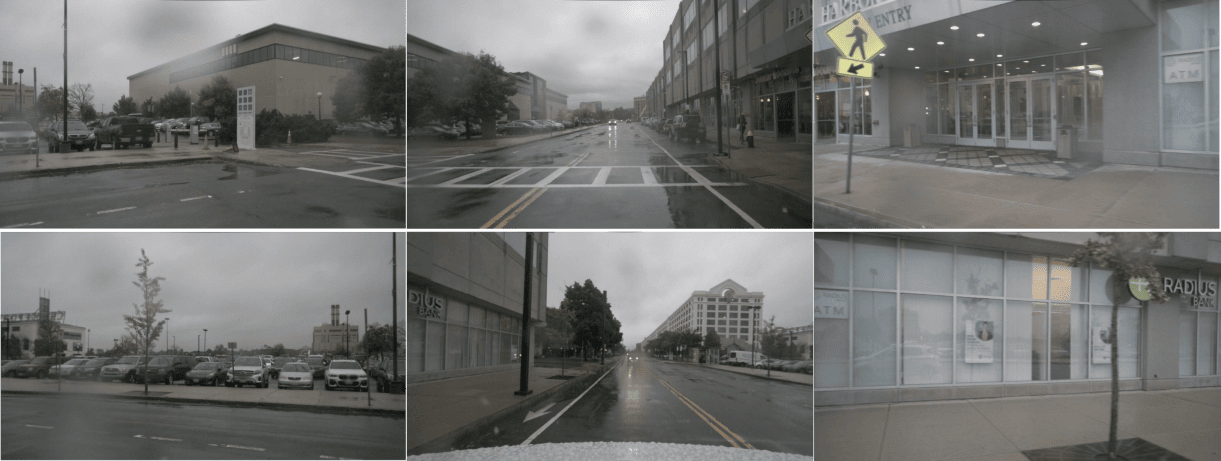
\includegraphics[width=0.9\linewidth]{src/description_exp1.png}
\end{center}

\vspace{1ex}

\noindent\textbf{\textcolor{purple}{Scene Style:}}
\begin{itemize}[leftmargin=15pt, itemsep=2pt]
    \item \textcolor{blue}{Time of the day}: daytime, with diffused lighting due to cloud cover
    \item \textcolor{blue}{Weather}: light to moderate rain, as indicated by raindrops on the camera lens and wet pavement
    \item \textcolor{blue}{Surrounding environment}: urban street flanked by mixed-use buildings and parking areas
    \item \textcolor{blue}{Road condition}: long, straight, two-lane road with clearly marked crosswalks and lane dividers; visibly slick from rainfall


\end{itemize}

\noindent\textbf{\textcolor{purple}{Foreground Objects:}}
\begin{itemize}[leftmargin=15pt, itemsep=2pt]
  \item \textcolor{blue}{Cars (left side)}: a variety of parked vehicles, including a dark pickup truck, compact sedans, SUVs, and so on, aligned parallel along the sidewalk; some cars have reflections on the wet ground
  \item \textcolor{blue}{Cars (right side)}: several vehicles parked curbside in front of commercial buildings, including economy cars to midsize SUVs
  \item \textcolor{blue}{Pedestrian}: an individual wearing a bright orange reflective safety vest and holding a red umbrella, standing near a crosswalk, suggesting a crossing action in progress
  \item \textcolor{blue}{Traffic cone}: bright orange cone placed on the sidewalk near the edge of a parking entrance, likely for safety or to reserve space
  \item \textcolor{blue}{Traffic sign}: a yellow pedestrian crossing sign mounted on a pole; the sign is positioned close to a glass-door building entrance
\end{itemize}

\noindent\textbf{\textcolor{purple}{Background Elements:}}
\begin{itemize}[leftmargin=15pt, itemsep=2pt]
  \item \textcolor{blue}{Road}: appears dark and glossy due to recent rainfall; lane markings and crosswalks are clearly visible
  \item \textcolor{blue}{Sidewalk}: wide, concrete sidewalks run alongside the road, bordered by planters and lined with trees
  \item \textcolor{blue}{Buildings}: prominent structures include multi-level modern commercial buildings with large glass façades
  \item \textcolor{blue}{Trees}: scattered urban landscaping includes small trees planted at regular intervals, offering a touch of greenery
  \item \textcolor{blue}{Car Parking}: multiple designated parking areas, some directly along the street and others within enclosed lots
  \item \textcolor{blue}{Crosswalk}: wide white-striped pedestrian crossings present at intersections
  \item \textcolor{blue}{Streetlights}: installed at intervals along the road to provide visibility during low-light conditions
\end{itemize}

\noindent\textbf{\textcolor{purple}{Scene-Graph Layout:}}
\begin{center}
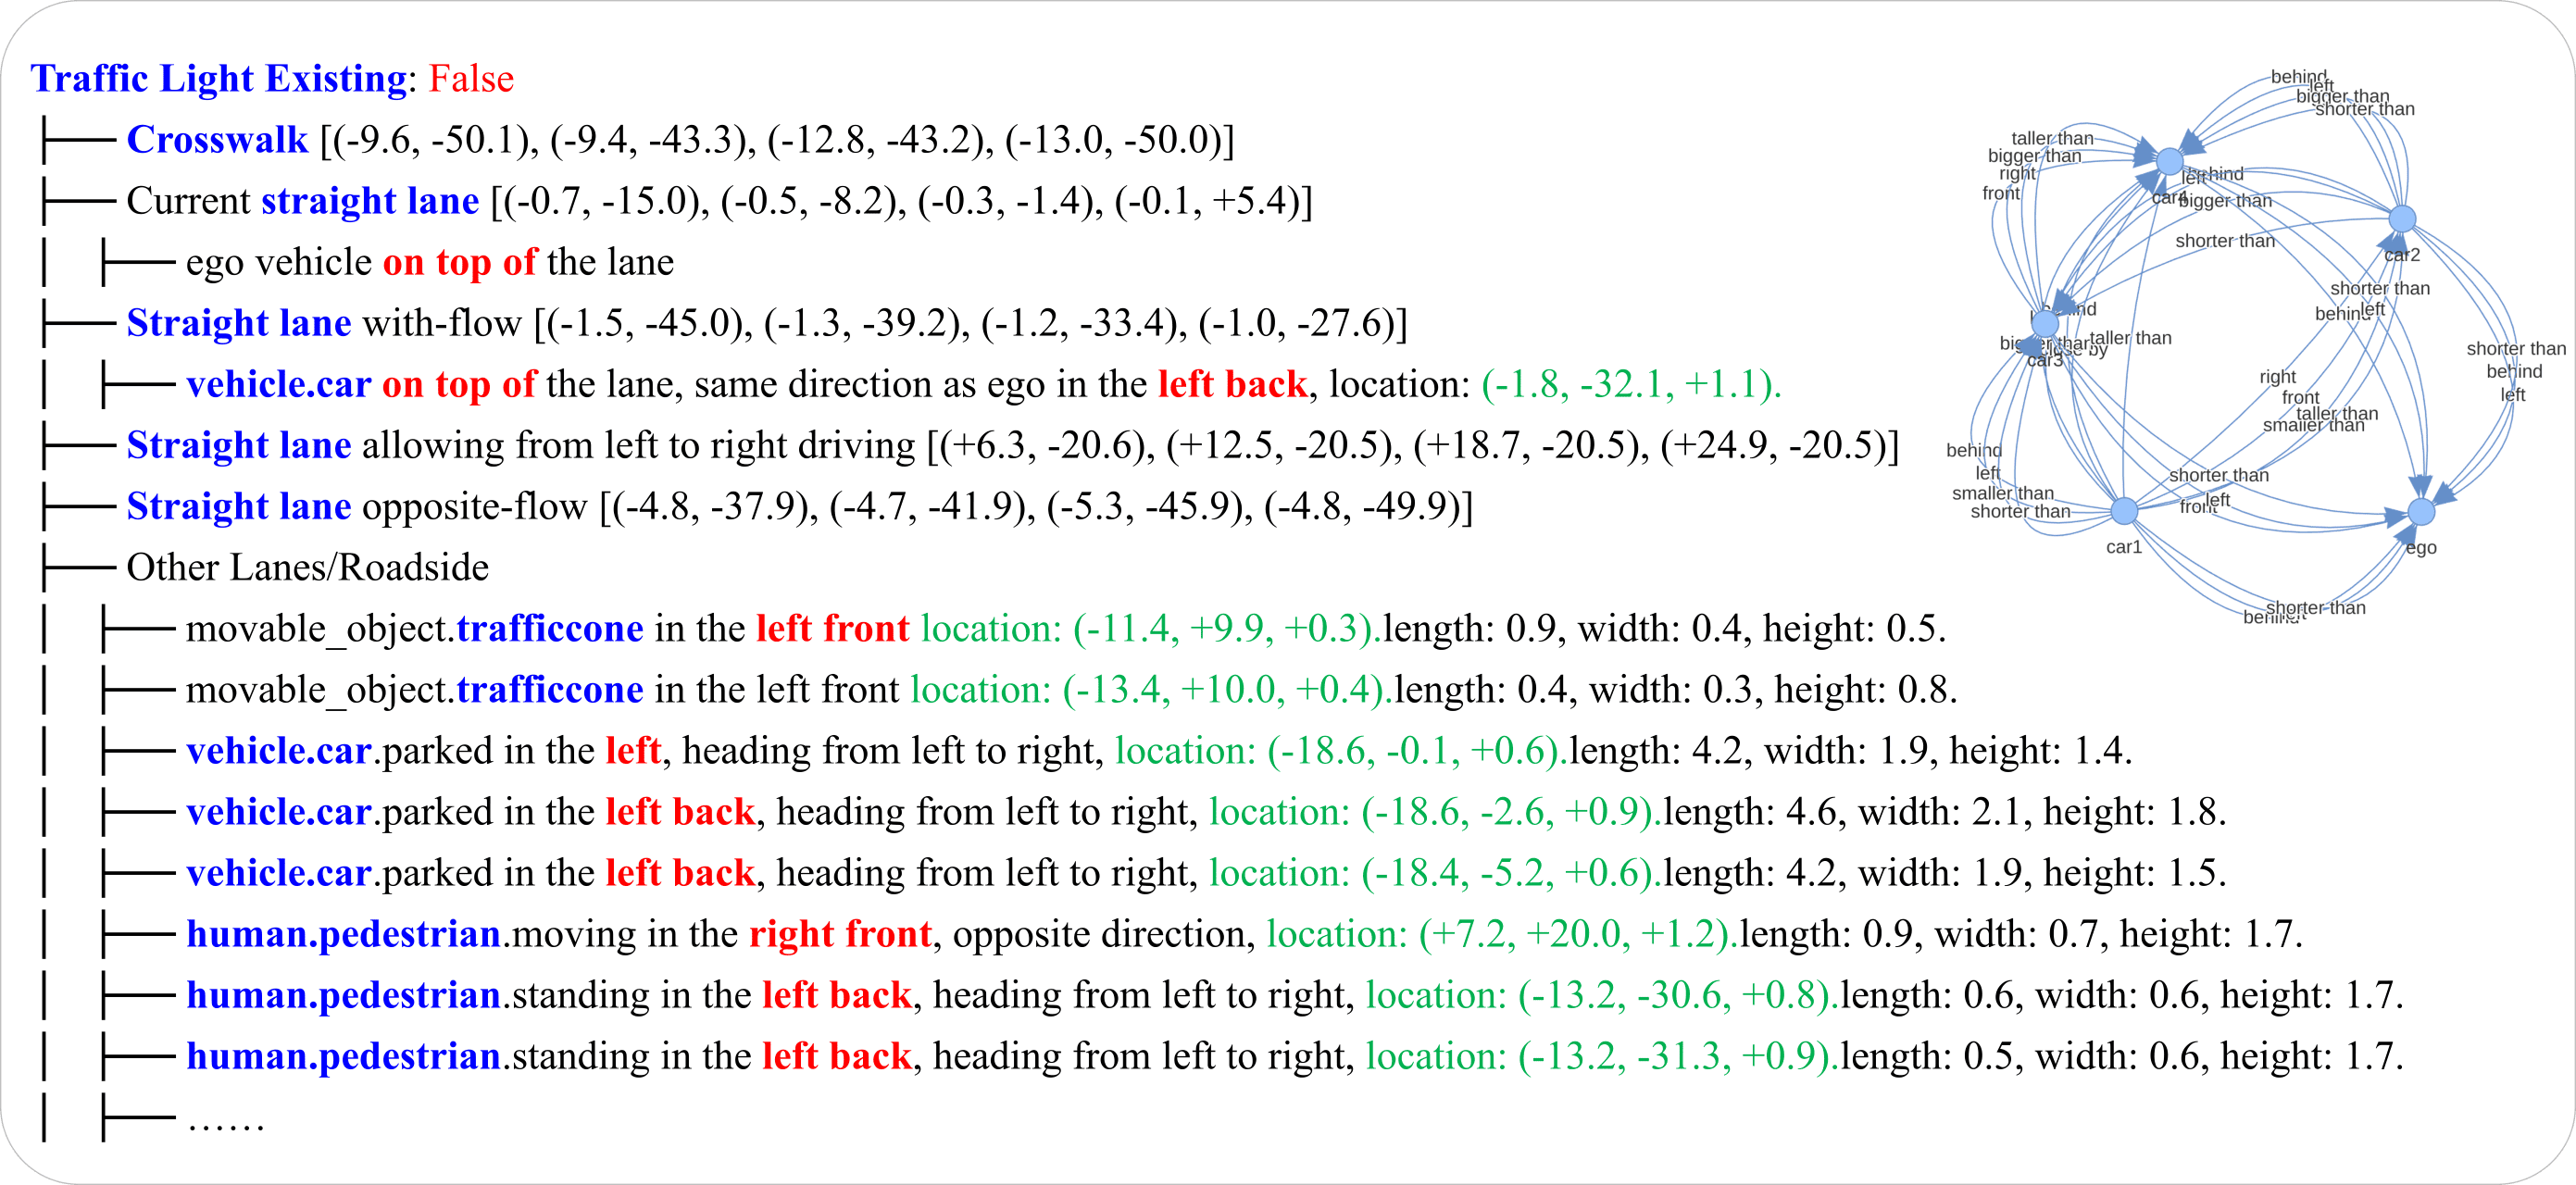
\includegraphics[width=0.98\linewidth]{src/layout1.png}
\end{center}


\noindent\textbf{\textcolor{purple}{Abstract Description:}}
\begin{itemize}[leftmargin=15pt, itemsep=2pt]
  \item \textcolor{gray!10!black}{The scene shows a rainy day on an urban expressway with wet roads reflecting light. Numerous cars are parked on both sides of the street, and a pedestrian in a bright orange safety vest is near the crosswalk. The background features multi-story commercial buildings with large windows, trees lining the sidewalk, and various signage. Streetlights are visible, and the area is marked with crosswalks and lane lines, creating a realistic and structured urban driving scene.}
\end{itemize}

\end{tcolorbox}

\tcbset{
  myboxstyle/.style={
    boxrule=1pt,
    boxsep=2pt,
    colback=gray!5,
    fontupper=\scriptsize,
    fonttitle=\color{black},
    title=Scene Description Example,
    coltitle=black,
    colframe=black,
    colbacktitle=blue!10,
    breakable
  }
}

\tcbset{
  myjsonbox/.style={
    enhanced,
    colframe=gray!50,
    colback=white,
    fonttitle=\small\color{white},
    boxrule=0.8pt,
    arc=4pt,
    left=4pt,
    right=4pt,
    top=4pt,
    bottom=4pt,
    boxsep=5pt,
    listing only,
    listing options={
      language=json,
      basicstyle=\scriptsize\ttfamily,
      keywordstyle=\color{blue},
      stringstyle=\color{orange!90!black},
      commentstyle=\color{gray},
      morekeywords={true,false,null},
      literate=%
        *{,}{{\textcolor{red}{,}}}{1}%
         {:}{{\textcolor{red}{:}}}{1}%
         {\{}{{\textcolor{red}{\{}}}{1}%
         {\}}{{\textcolor{red}{\}}}}{1}%
    },
    breakable,
  }
}

\lstdefinelanguage{json}{
    basicstyle=\ttfamily\footnotesize,
    showstringspaces=false,
    breaklines=true,
    breakatwhitespace=true,
    morestring=[b]",
    stringstyle=\color{orange!90!black},
    morecomment=[s]{/*}{*/},
    commentstyle=\color{gray},
    morekeywords={true,false,null},
    keywordstyle=\color{blue},
    literate=%
      *{,}{{\textcolor{red}{,}}}{1}%
       {:}{{\textcolor{red}{:}}}{1}%
       {\{}{{\textcolor{red}{\{}}}{1}%
       {\}}{{\textcolor{red}{\}}}}{1}%
}




\begin{tcolorbox}[myboxstyle]

\begin{center}
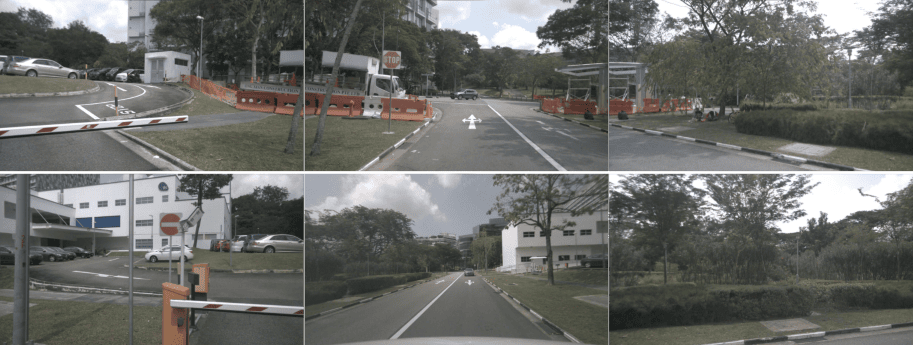
\includegraphics[width=0.9\linewidth]{src/description_exp2.png}
\end{center}

\vspace{1ex}

\noindent\textbf{\textcolor{purple}{Scene Style:}}
\begin{itemize}[leftmargin=15pt, itemsep=2pt]
    \item \textcolor{blue}{Time of the day}: bright daytime with clear shadows, indicating direct sunlight and good visibility
    \item \textcolor{blue}{Weather}: sunny with partly cloudy skies; no signs of precipitation or poor visibility
    \item \textcolor{blue}{Surrounding environment}: suburban campus or business park-like area with a mix of roadways, pedestrian paths, and landscaped
    \item \textcolor{blue}{Road condition}: smooth asphalt with a gentle curve transitioning into a straight segment




\end{itemize}

\noindent\textbf{\textcolor{purple}{Foreground Objects:}}
\begin{itemize}[leftmargin=15pt, itemsep=2pt]
  \item \textcolor{blue}{Barriers (construction zone)}: bright orange modular barriers clearly indicating a temporarily restricted area
  \item \textcolor{blue}{Truck (construction zone)}: a white construction truck with visible text parked adjacent to the barriers
  \item \textcolor{blue}{Stop sign (construction zone)}: standard red octagonal stop sign mounted on a metallic pole, reinforcing right-of-way rules
  \item \textcolor{blue}{Entrance barrier}:  red and white striped boom barrier at two vehicle access points, indicating controlled entry
  \item \textcolor{blue}{Cars}: silver sedan (parked at curve near the booth); black sedan (alongside silver); dark-colored sedan (moving towards camera, on central lane); red and silver vehicles (visible in side/rear view near building and behind the no-entry sign)
  \item \textcolor{blue}{Seated pedestrian}: a person is resting on the grassy area near the right side of the road, shaded by trees
\end{itemize}

\noindent\textbf{\textcolor{purple}{Background Elements:}}
\begin{itemize}[leftmargin=15pt, itemsep=2pt]
  \item \textcolor{blue}{Road}: dual-lane road with center markings and white directional arrows
  \item \textcolor{blue}{Sidewalk}: paved pathways flanked by grass and shrubs on both sides of the road
  \item \textcolor{blue}{Buildings}: main visible structure is a multi-story white facility with large windows and blue signage
  \item \textcolor{blue}{Vegetation}: tall green trees forming canopy along both sides of the road, sculpted bushes reinforce the planned landscape design
  \item \textcolor{blue}{Car Parking}: clearly delineated lot visible on the left, populated with multiple parked cars
  \item \textcolor{blue}{Traffic Signage}: a “No Entry” (red circle with horizontal white bar) sign prominently displayed at an access control gate
\end{itemize}


\noindent\textbf{\textcolor{purple}{Scene-Graph Layout:}}
\begin{center}
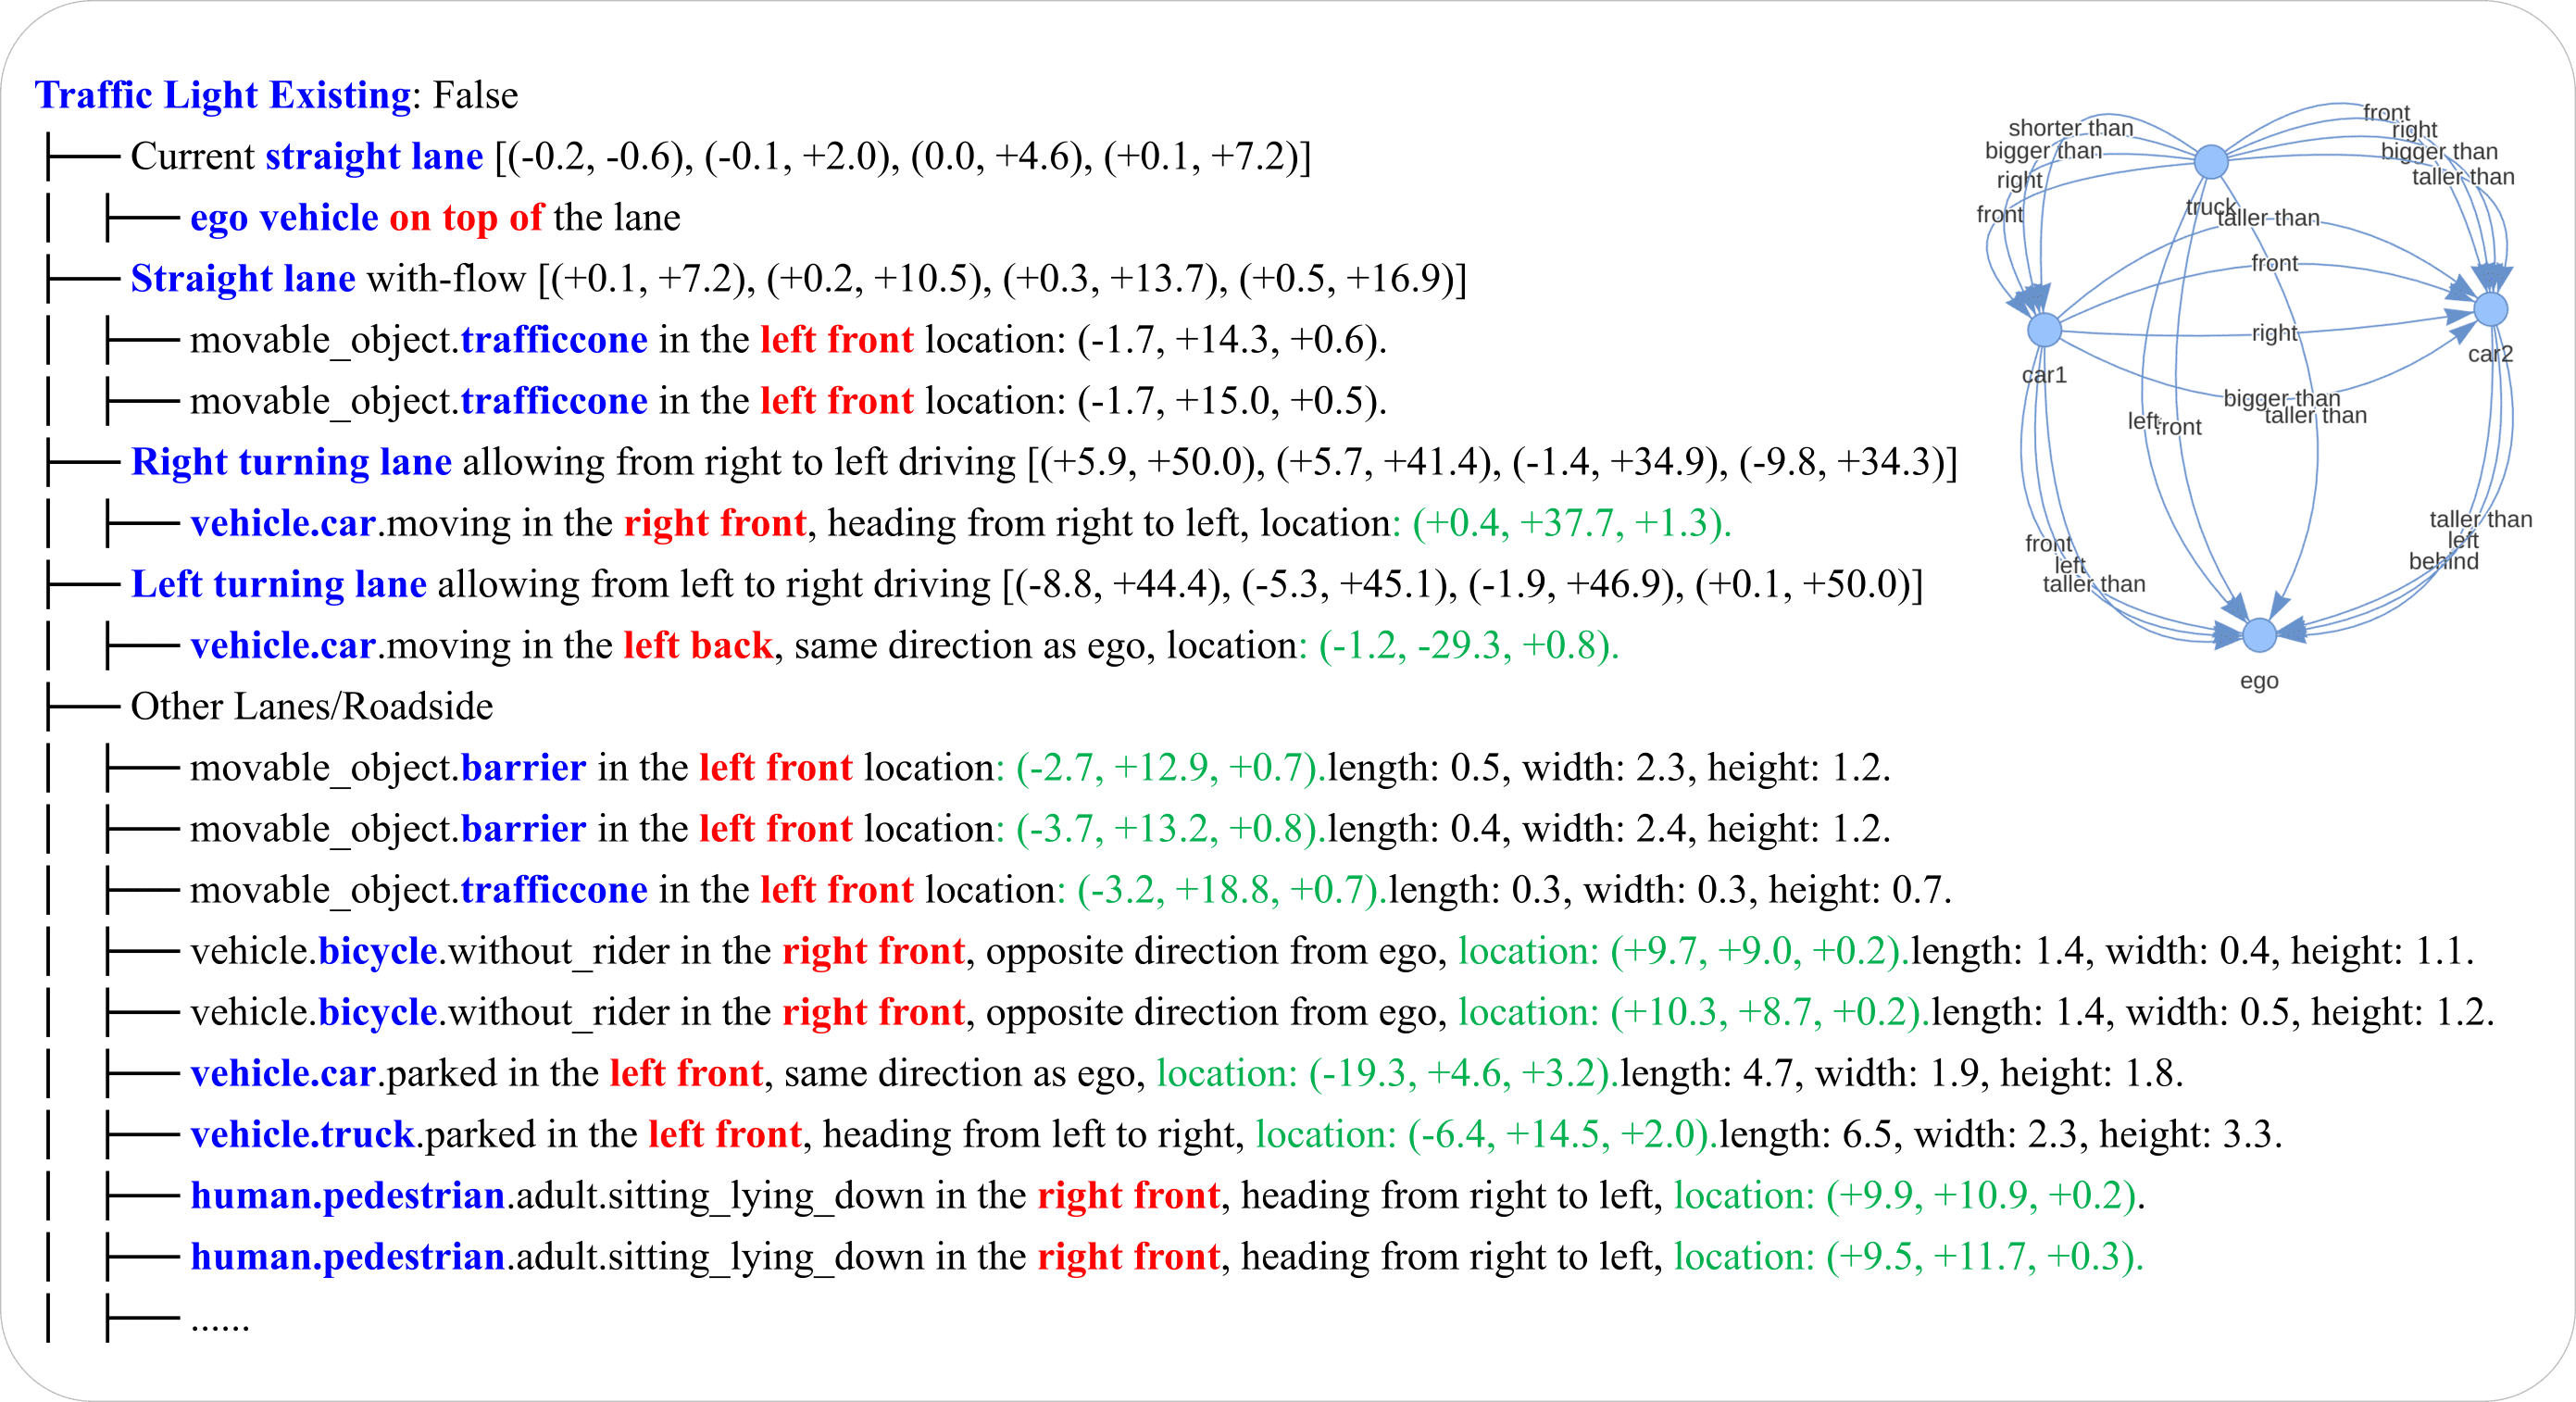
\includegraphics[width=0.98\linewidth]{src/layout2.png}
\end{center}


\noindent\textbf{\textcolor{purple}{Abstract Description:}}
\begin{itemize}[leftmargin=15pt, itemsep=2pt]
  \item \textcolor{gray!10!black}{The scene shows a sunny day in a suburban area with a mix of urban infrastructure and greenery. The road curves slightly before straightening out, with construction barriers and a stop sign indicating ongoing work. Several cars are parked along the roadside, while others are in motion. A pedestrian is seated on the grass near the right-rear view, and there are trees and buildings in the background. The road appears well-maintained, with clear lane markings and a mix of open spaces and developed areas.}
\end{itemize}

\end{tcolorbox}



\clearpage
\section{Additional Quantitative Results}
\begin{table*}[!t]
  \centering
  % ==== Text-only Ablation ====
  \begin{minipage}[t]{0.48\textwidth}
    \centering
    \setlength\tabcolsep{3pt}
    \caption{Ablation on text-only generation.}
    \vspace{0.5em}
    \resizebox{\linewidth}{!}{
      \begin{tabular}{l|c|cc|cc}
        \toprule
        \multirow{2}{*}{\textbf{Variants}} & \multirow{2}{*}{\textbf{FID$\downarrow$}} &
        \multicolumn{2}{c|}{\textbf{3DOD}} &
        \multicolumn{2}{c}{\textbf{BEVSeg mIoU (\%)}} \\
        \cline{3-6}
         &  & mAP$\uparrow$ & NDS$\uparrow$ & Road$\uparrow$ & Vehicle$\uparrow$ \\
        \midrule
        \rowcolor{gray!10} Full Model & \textbf{11.29} & \textbf{16.28} & \textbf{26.26} & \textbf{66.48} & \textbf{29.76} \\
        Text Only & 20.74 & 2.13 & 5.34 & 28.32 & 7.49 \\
        \bottomrule
      \end{tabular}
    }
    \label{tab:ablation_spatial}
  \end{minipage}
  \hfill
  % ==== Layout Type Ablation ====
  \begin{minipage}[t]{0.51\textwidth}
    \centering
    \setlength\tabcolsep{3pt}
    \caption{Ablation on input layout types.}
    \vspace{0.5em}
    \resizebox{\linewidth}{!}{
      \begin{tabular}{l|c|cc|cc}
        \toprule
        \multirow{2}{*}{\textbf{Input Layout}} & \multirow{2}{*}{\textbf{FID$\downarrow$}} &
        \multicolumn{2}{c|}{\textbf{3DOD}} &
        \multicolumn{2}{c}{\textbf{BEVSeg mIoU (\%)}} \\
        \cline{3-6}
         &  & mAP$\uparrow$ & NDS$\uparrow$ & Road$\uparrow$ & Vehicle$\uparrow$ \\
        \midrule
        \rowcolor{gray!10} Semantic Map & \textbf{11.29} & \textbf{16.28} & \textbf{26.26} & \textbf{66.48} & \textbf{29.76} \\
        Vector Map & 12.07 & 15.73 & 25.84 & 65.17 & 28.38 \\
        \bottomrule
      \end{tabular}
    }
    \label{tab:ablation_layout}
  \end{minipage}
  \vspace{-3mm}
\end{table*}

\begin{table*}[!t]
  \centering
  % ==== Layout Noise Ablation ====
  \begin{minipage}[t]{0.61\textwidth}
    \centering
    \setlength\tabcolsep{3pt}
    \caption{\textbf{Robustness to layout noise.} Performance under noisy layout shows graceful degradation across stages.}
    \vspace{0.5em}
    \resizebox{\linewidth}{!}{
      \begin{tabular}{l|cc|c|cc|cc}
        \toprule
        \multirow{2}{*}{\textbf{Layout}} &
        \multicolumn{2}{c|}{\textbf{OccGen}} &
        \textbf{ImgGen} &
        \multicolumn{2}{c|}{\textbf{3DOD}} &
        \multicolumn{2}{c}{\textbf{BEVSeg mIoU(\%)}} \\
        \cline{2-8}
         & FID$^{3\text{D}}\downarrow$ & F$^{3\text{D}}\uparrow$ & FID$\downarrow$ &
         mAP$\uparrow$ & NDS$\uparrow$ & Road$\uparrow$ & Vehicle$\uparrow$ \\
        \midrule
        \rowcolor{gray!10} Clean & \textbf{258.8} & \textbf{0.778} & \textbf{11.29} & \textbf{16.28} & \textbf{26.26} & \textbf{66.48} & \textbf{29.76} \\
        Noisy & 276.3 & 0.742 & 12.47 & 14.87 & 25.02 & 65.28 & 28.44 \\
        \bottomrule
      \end{tabular}
    }
    \label{tab:ablation_noise}
  \end{minipage}
  \hfill
  % ==== Inference Cost ====
  \begin{minipage}[t]{0.37\textwidth}
    \centering
    \setlength\tabcolsep{4pt}
    \caption{\textbf{Inference efficiency} of each stage on a single RTX~A6000.}
    \vspace{0.5em}
    \resizebox{\linewidth}{!}{
      \begin{tabular}{l|c|c|c}
        \toprule
        \textbf{Stage} & \textbf{Steps} & \textbf{Time (s)} & \textbf{GPU (GB)} \\
        \midrule
        LayoutGen & 50 & 0.15 & 1.0 \\
        OccGen & 20 & 3.25 & 7.7 \\
        ImgGen & 20 & 2.30 & 7.0 \\
        \bottomrule
      \end{tabular}
    }
    \label{tab:inference_cost}
  \end{minipage}
  \vspace{-3mm}
\end{table*}


\subsection{Effect of Spatial Conditioning}
We evaluate the role of spatial conditioning using a \textit{text-only} variant that removes all spatial inputs (layout maps, object boxes, and perspective maps) while retaining textual prompts. As shown in Table~\ref{tab:ablation_spatial}, the absence of spatial cues causes clear degradation in visual realism (FID $\uparrow$ 9.45) and spatial fidelity (Vehicle mIoU $\downarrow$ 22.27\%), underscoring the importance of spatial conditioning for maintaining geometric coherence and consistent scene alignment.


\subsection{Effect of Layout Type}
To examine different layout representations in our dual-mode controllability design, we compare two layout types: 1) \textit{BEV semantic maps} for fine-grained spatial control and 2) \textit{BEV vector maps} of object boxes and lanes for efficient customization. As shown in Table~\ref{tab:ablation_layout}, both yield geometrically accurate and visually coherent scenes, while semantic maps provide stronger spatial priors with slightly better realism and downstream performance. This confirms that both layout types are fully compatible with our pipeline, enabling flexible and effective scene control.


\subsection{Robustness and Efficiency}
To assess potential error accumulation in our cascaded generation pipeline, we conduct a noise-injection ablation by applying Gaussian perturbations (25\% probability) to the initial layout, including 3D box centers and lane coordinates. As shown in Table~\ref{tab:ablation_noise}, the pipeline degrades gracefully under noise, with only marginal drops in downstream metrics. This robustness arises from the multi-stage alignment design, where occupancy-rendered semantic and depth priors enforce geometric consistency, and overlap-aware extrapolation maintains spatial continuity.

We also report inference efficiency in Table~\ref{tab:inference_cost}. Each scene chunk is generated in about 6~seconds on a single RTX~A6000 GPU, showing that our system achieves a strong balance between robustness and computational efficiency for large-scale scene synthesis.

\begin{wraptable}{r}{0.43\textwidth}
\vspace{-6.5mm}
\centering
\renewcommand{\arraystretch}{1.1}
% \setlength{\tabcolsep}{2.5pt}
\caption{\textbf{Human preference study} comparing scene generation w/ and w/o RAG.}
\label{tab:ablation_rag}
\vspace{2mm}
\resizebox{\linewidth}{!}{
\begin{tabular}{lcc}
\toprule
\textbf{Criterion} & \textbf{RAG (\%)} & \textbf{Non-RAG (\%)} \\
\midrule
Diversity & \textbf{87} & 13 \\
Realism & \textbf{82} & 18 \\
Controllability & \textbf{74} & 26 \\
Phys. Plaus. & \textbf{66} & 34 \\
\midrule
\textbf{Overall} & \textbf{77} & 23 \\
\bottomrule
\end{tabular}
}
\vspace{-4mm}
\end{wraptable}

\subsection{Effect of Retrieval-Augmented Generation}
RAG enhances text-to-scene generation by expanding brief prompts into detailed scene descriptions through retrieving semantically related examples from a memory bank. This process transfers prior knowledge from similar scenes, improving layout accuracy and reducing user effort. Table~\ref{tab:ablation_rag} presents a human preference study in which ten participants evaluated 100 scene pairs generated with and without RAG across multiple criteria. The results show that RAG-based generation is consistently preferred (overall 77\% vs.\ 23\%), highlighting its effectiveness in grounding prompts and producing more diverse, realistic, and controllable scenes.

\clearpage
\section{Additional Qualitative Results}

\subsection{Conditional Occupancy and Image Generation}
Figure~\ref{fig:vis_result} presents additional conditional generation results, where layout conditions are used to synthesize multi-view images and 3D occupancy. These results demonstrate the effectiveness of our approach in generating coherent multi-modal outputs conditioned on low-level layout inputs. 
\vspace{-.5em}
\begin{figure}[H]
    \centering
    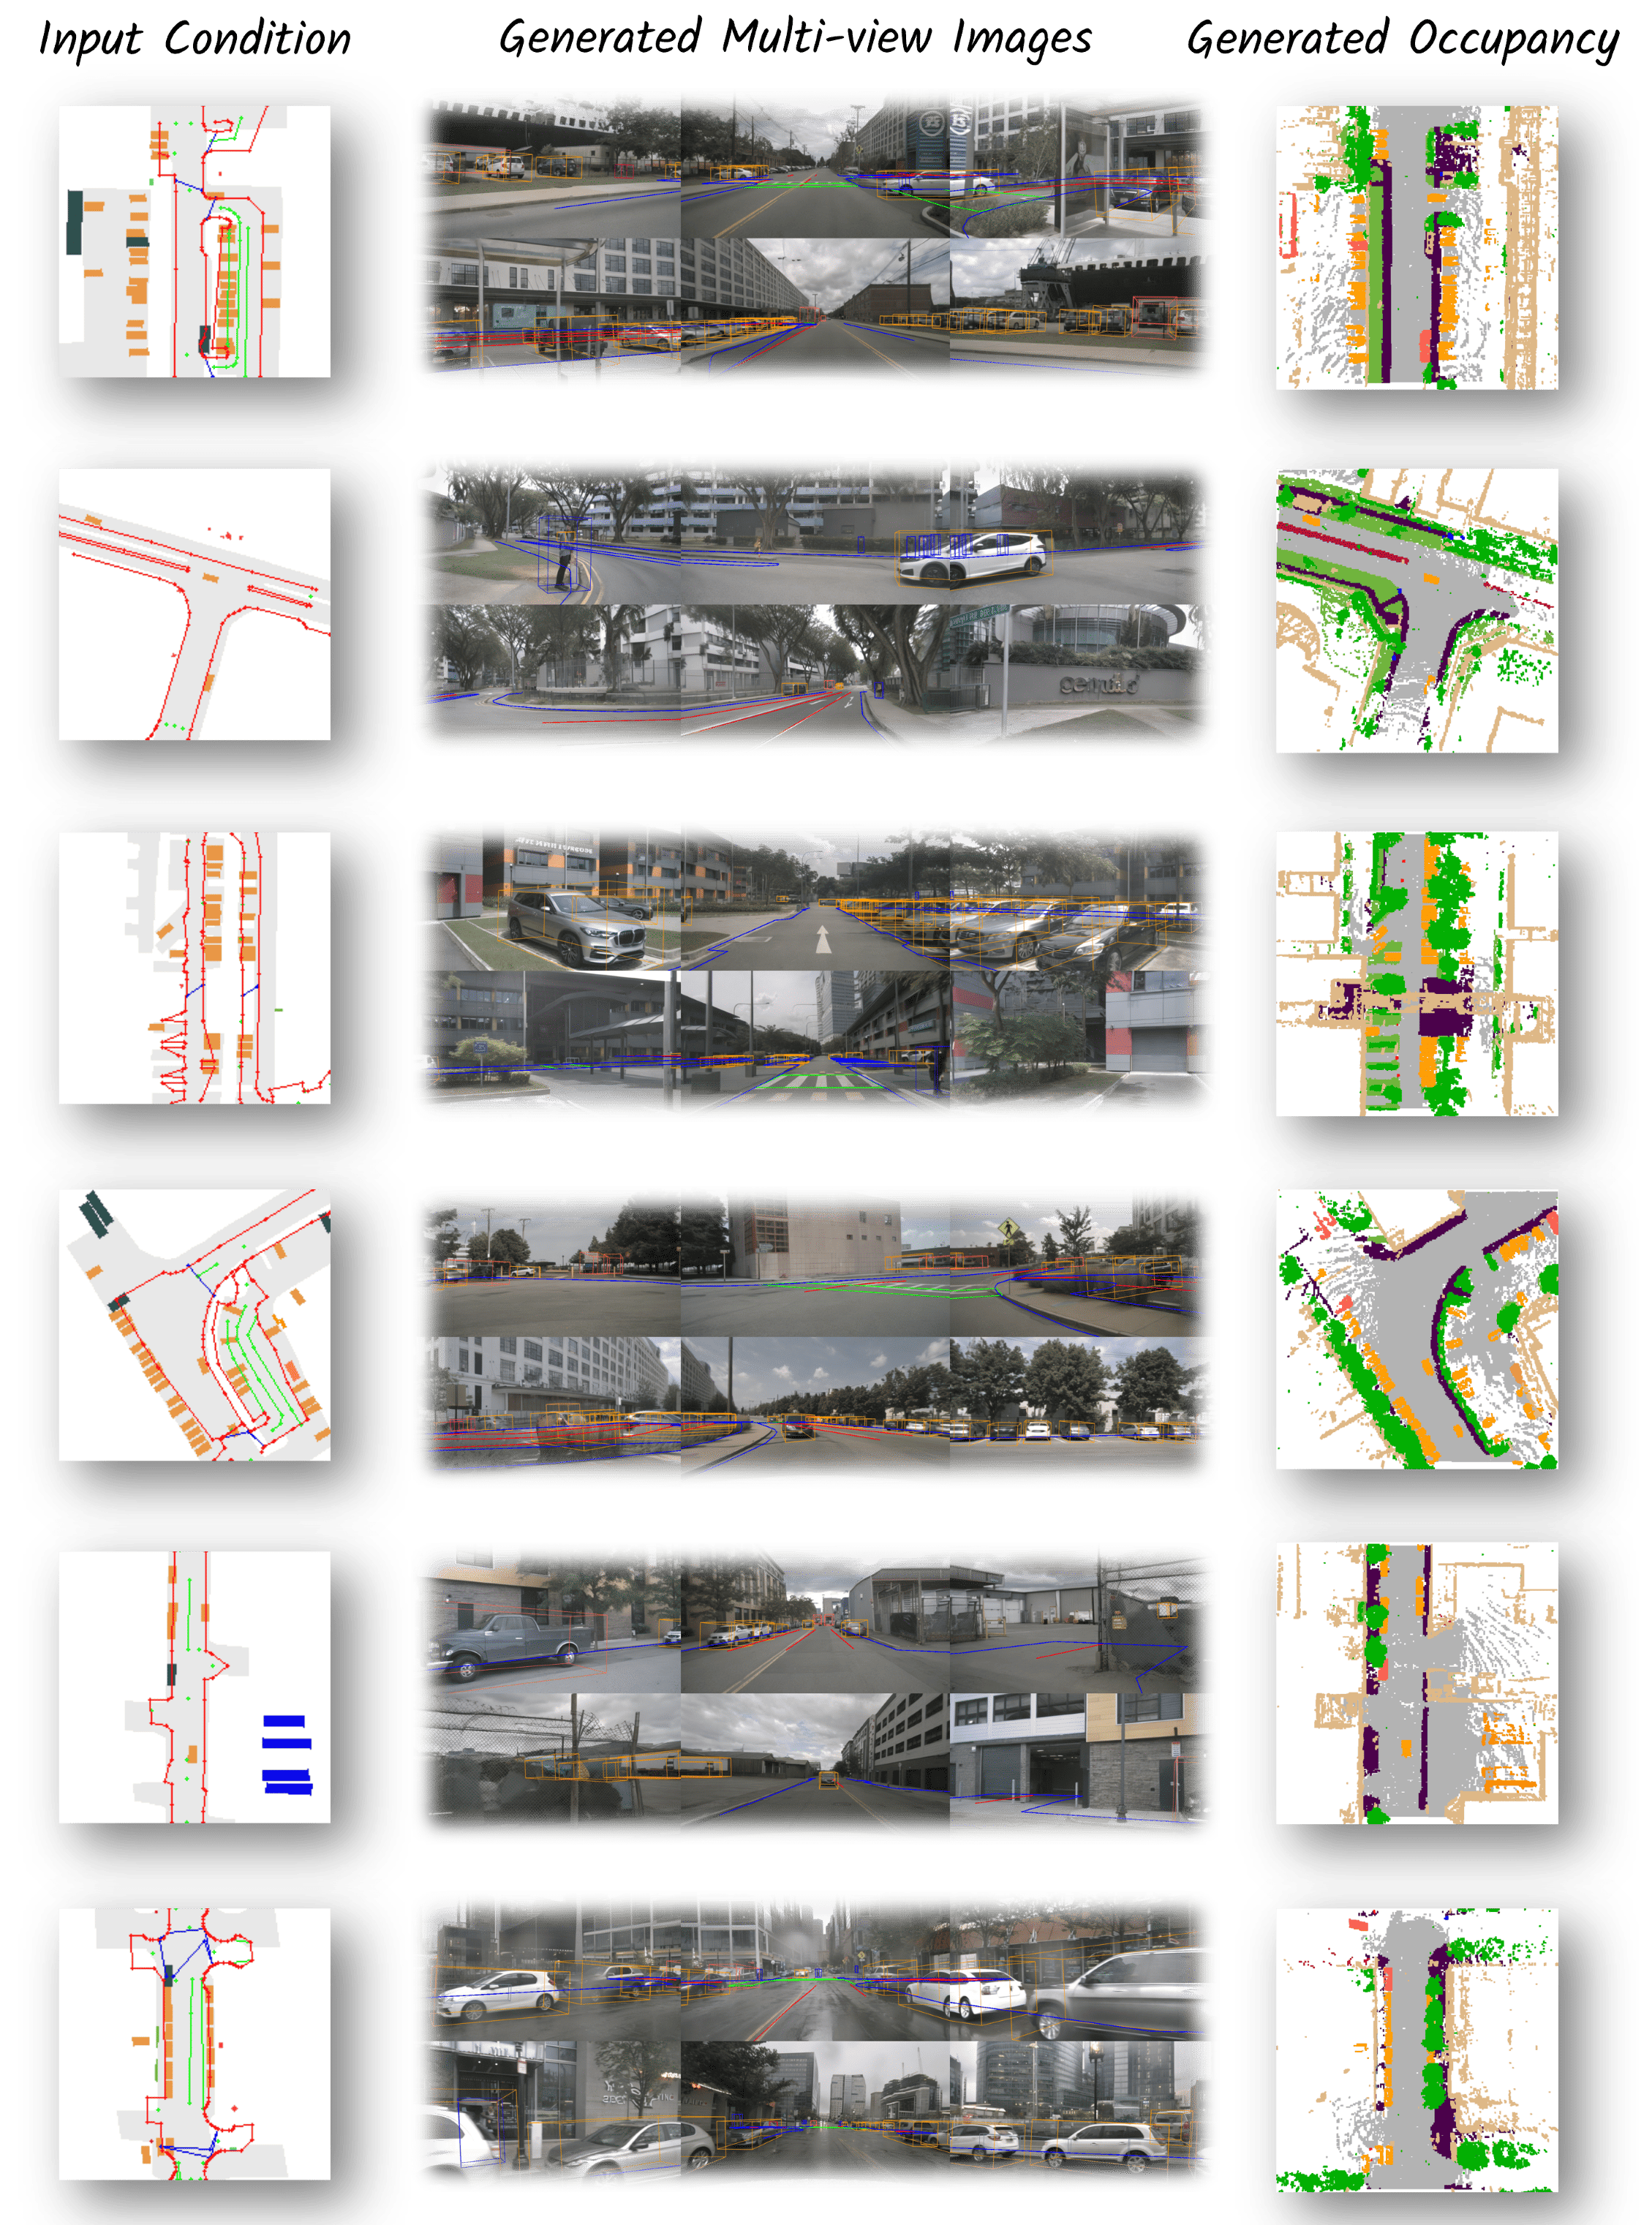
\includegraphics[width=0.98\textwidth]{src/vis_result.png}
    \vspace{-.5em}
    \caption{\textbf{Additional qualitative results of {\ours} on conditional occupancy and image generation.} These results demonstrate the model’s ability to generate semantically consistent and structurally accurate multi-modal outputs conditioned on layout inputs across diverse urban scenes.}
\label{fig:vis_result}
\vspace{-1mm}
\end{figure}

\input{figures/vis_text2scene_1}
\begin{figure}[t]
    \centering
    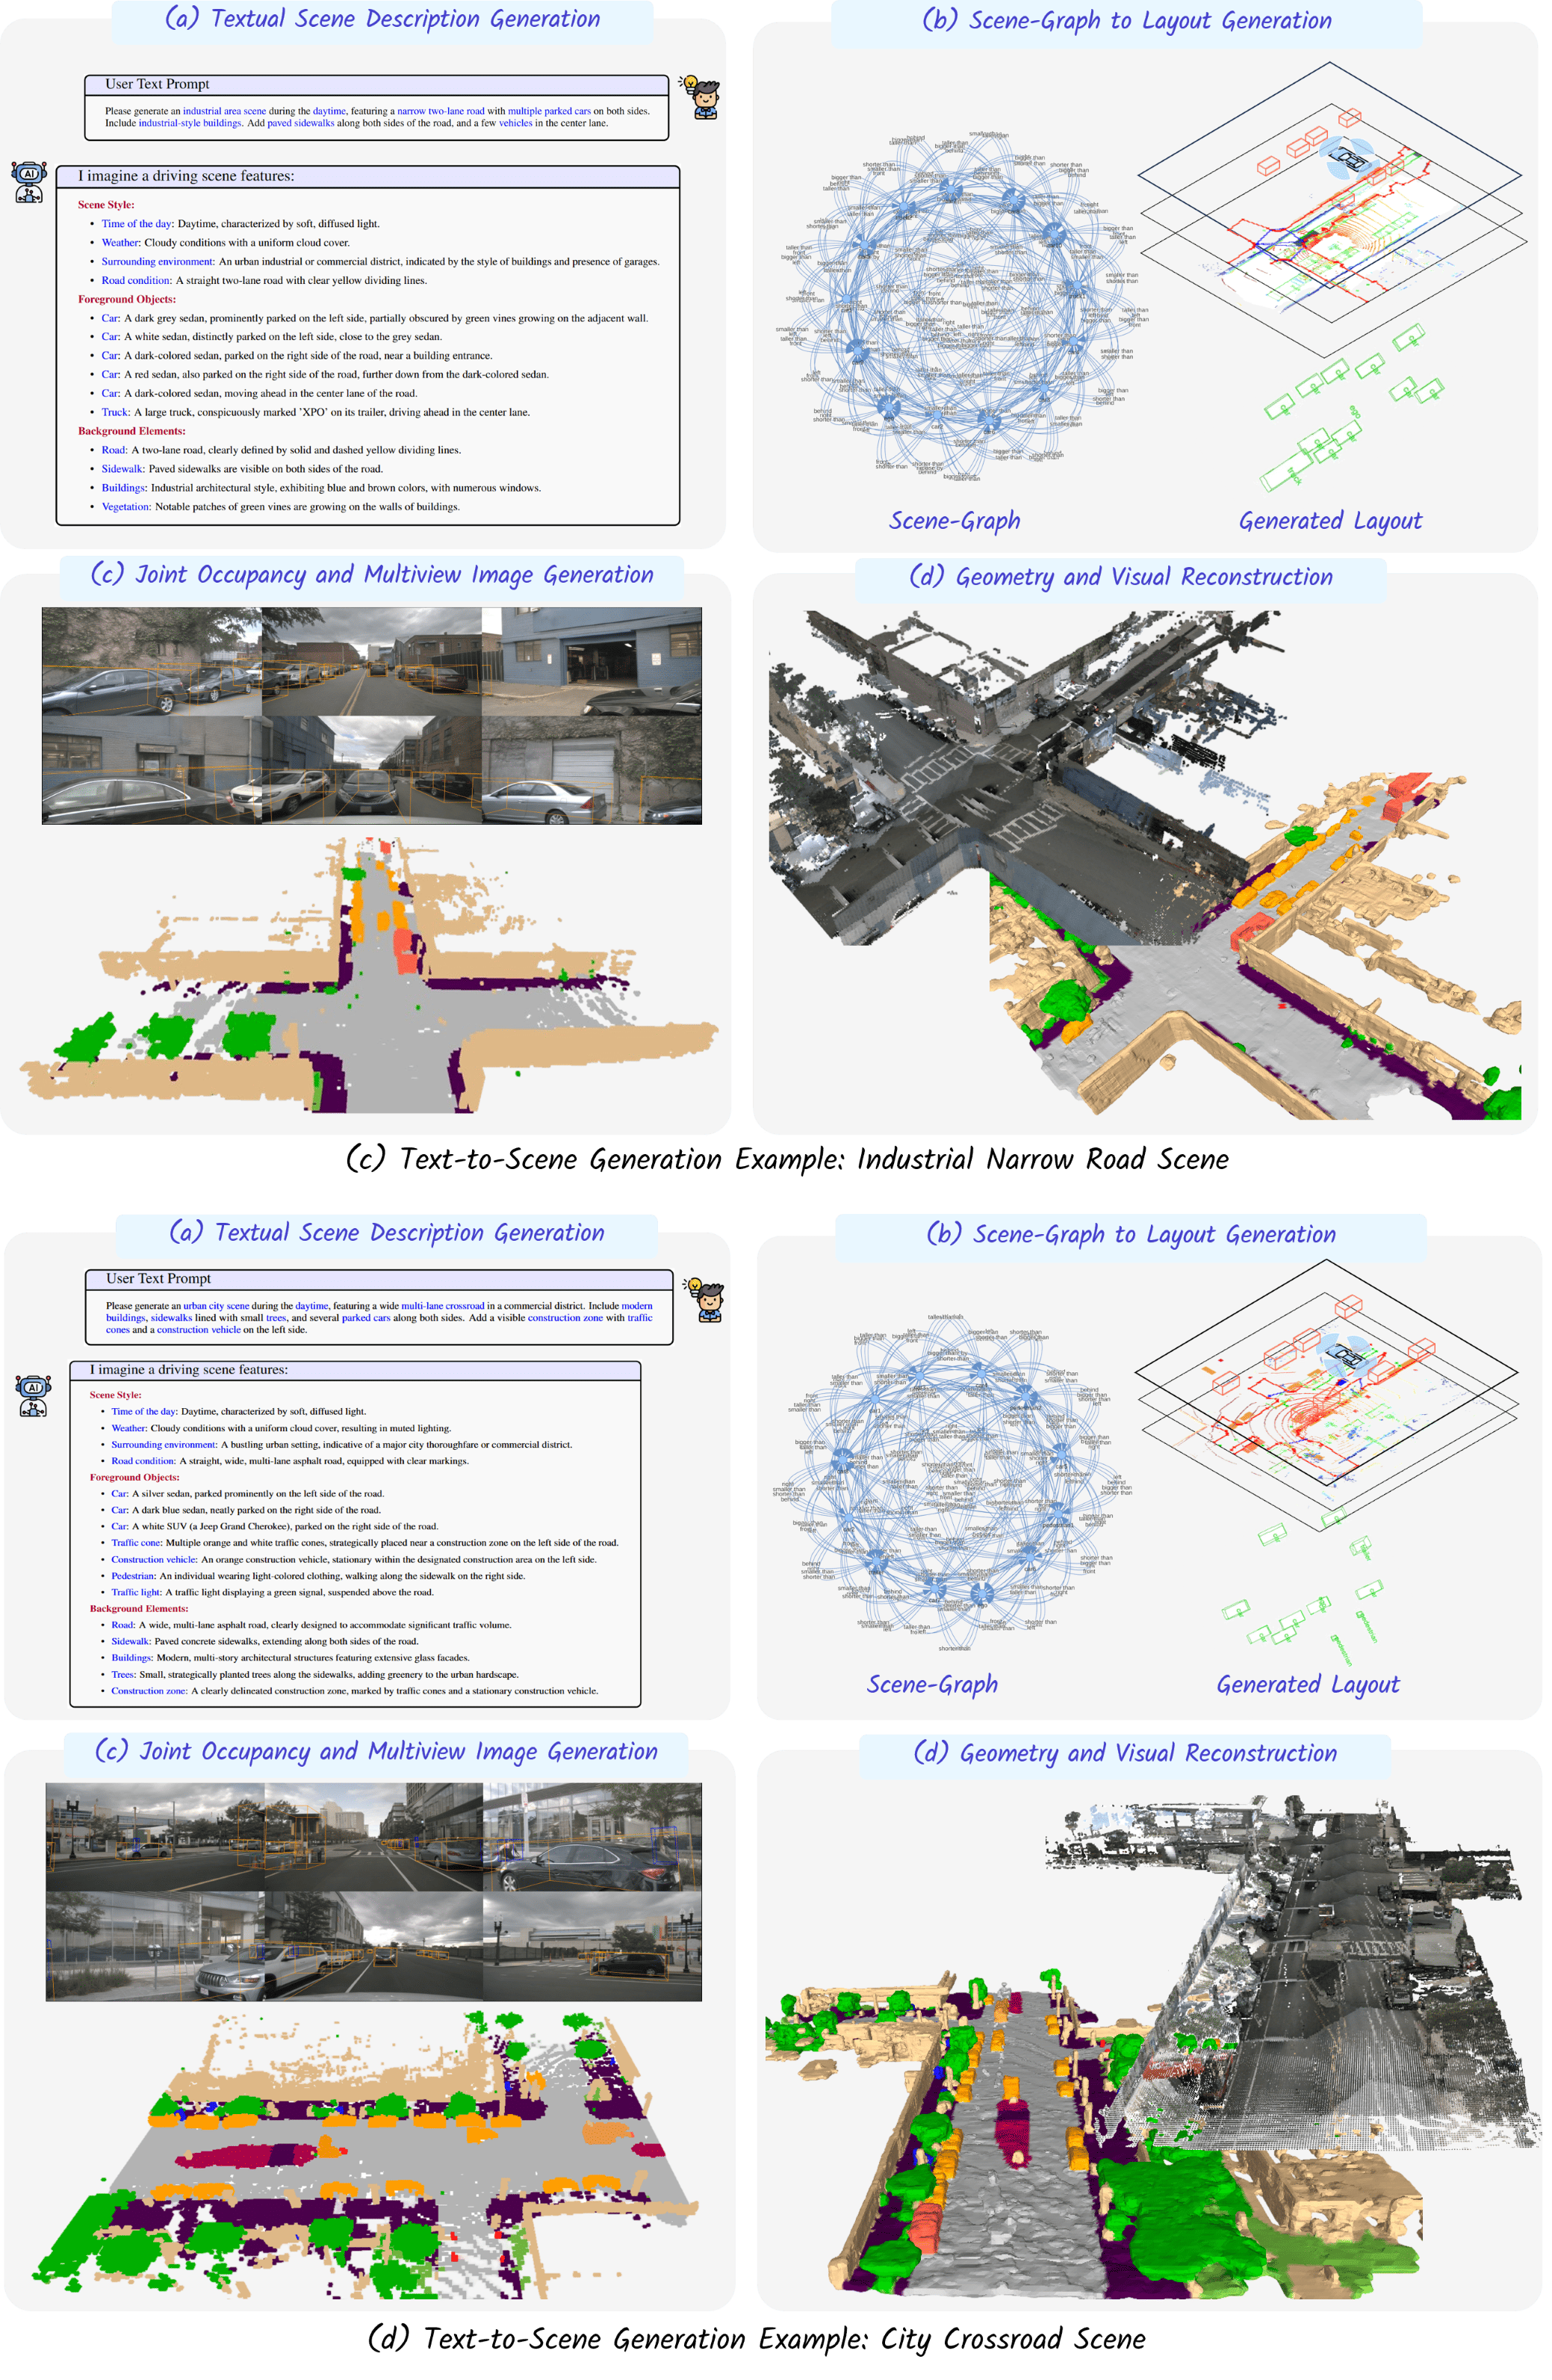
\includegraphics[width=1.0\textwidth]{src/text2scene_2.png}
    \vspace{-1.5em}
    \caption{\textbf{Qualitative results of the text-to-scene generation pipeline of {\ours}}. Starting from a user prompt, the system generates a plausible scene description, constructs the corresponding layout, synthesizes consistent occupancy and multi-view images, and finally performs 3D reconstruction.}
\label{fig:vis_text2scene_2}
\vspace{-1mm}
\end{figure}

\begin{figure}[t]
    \centering
    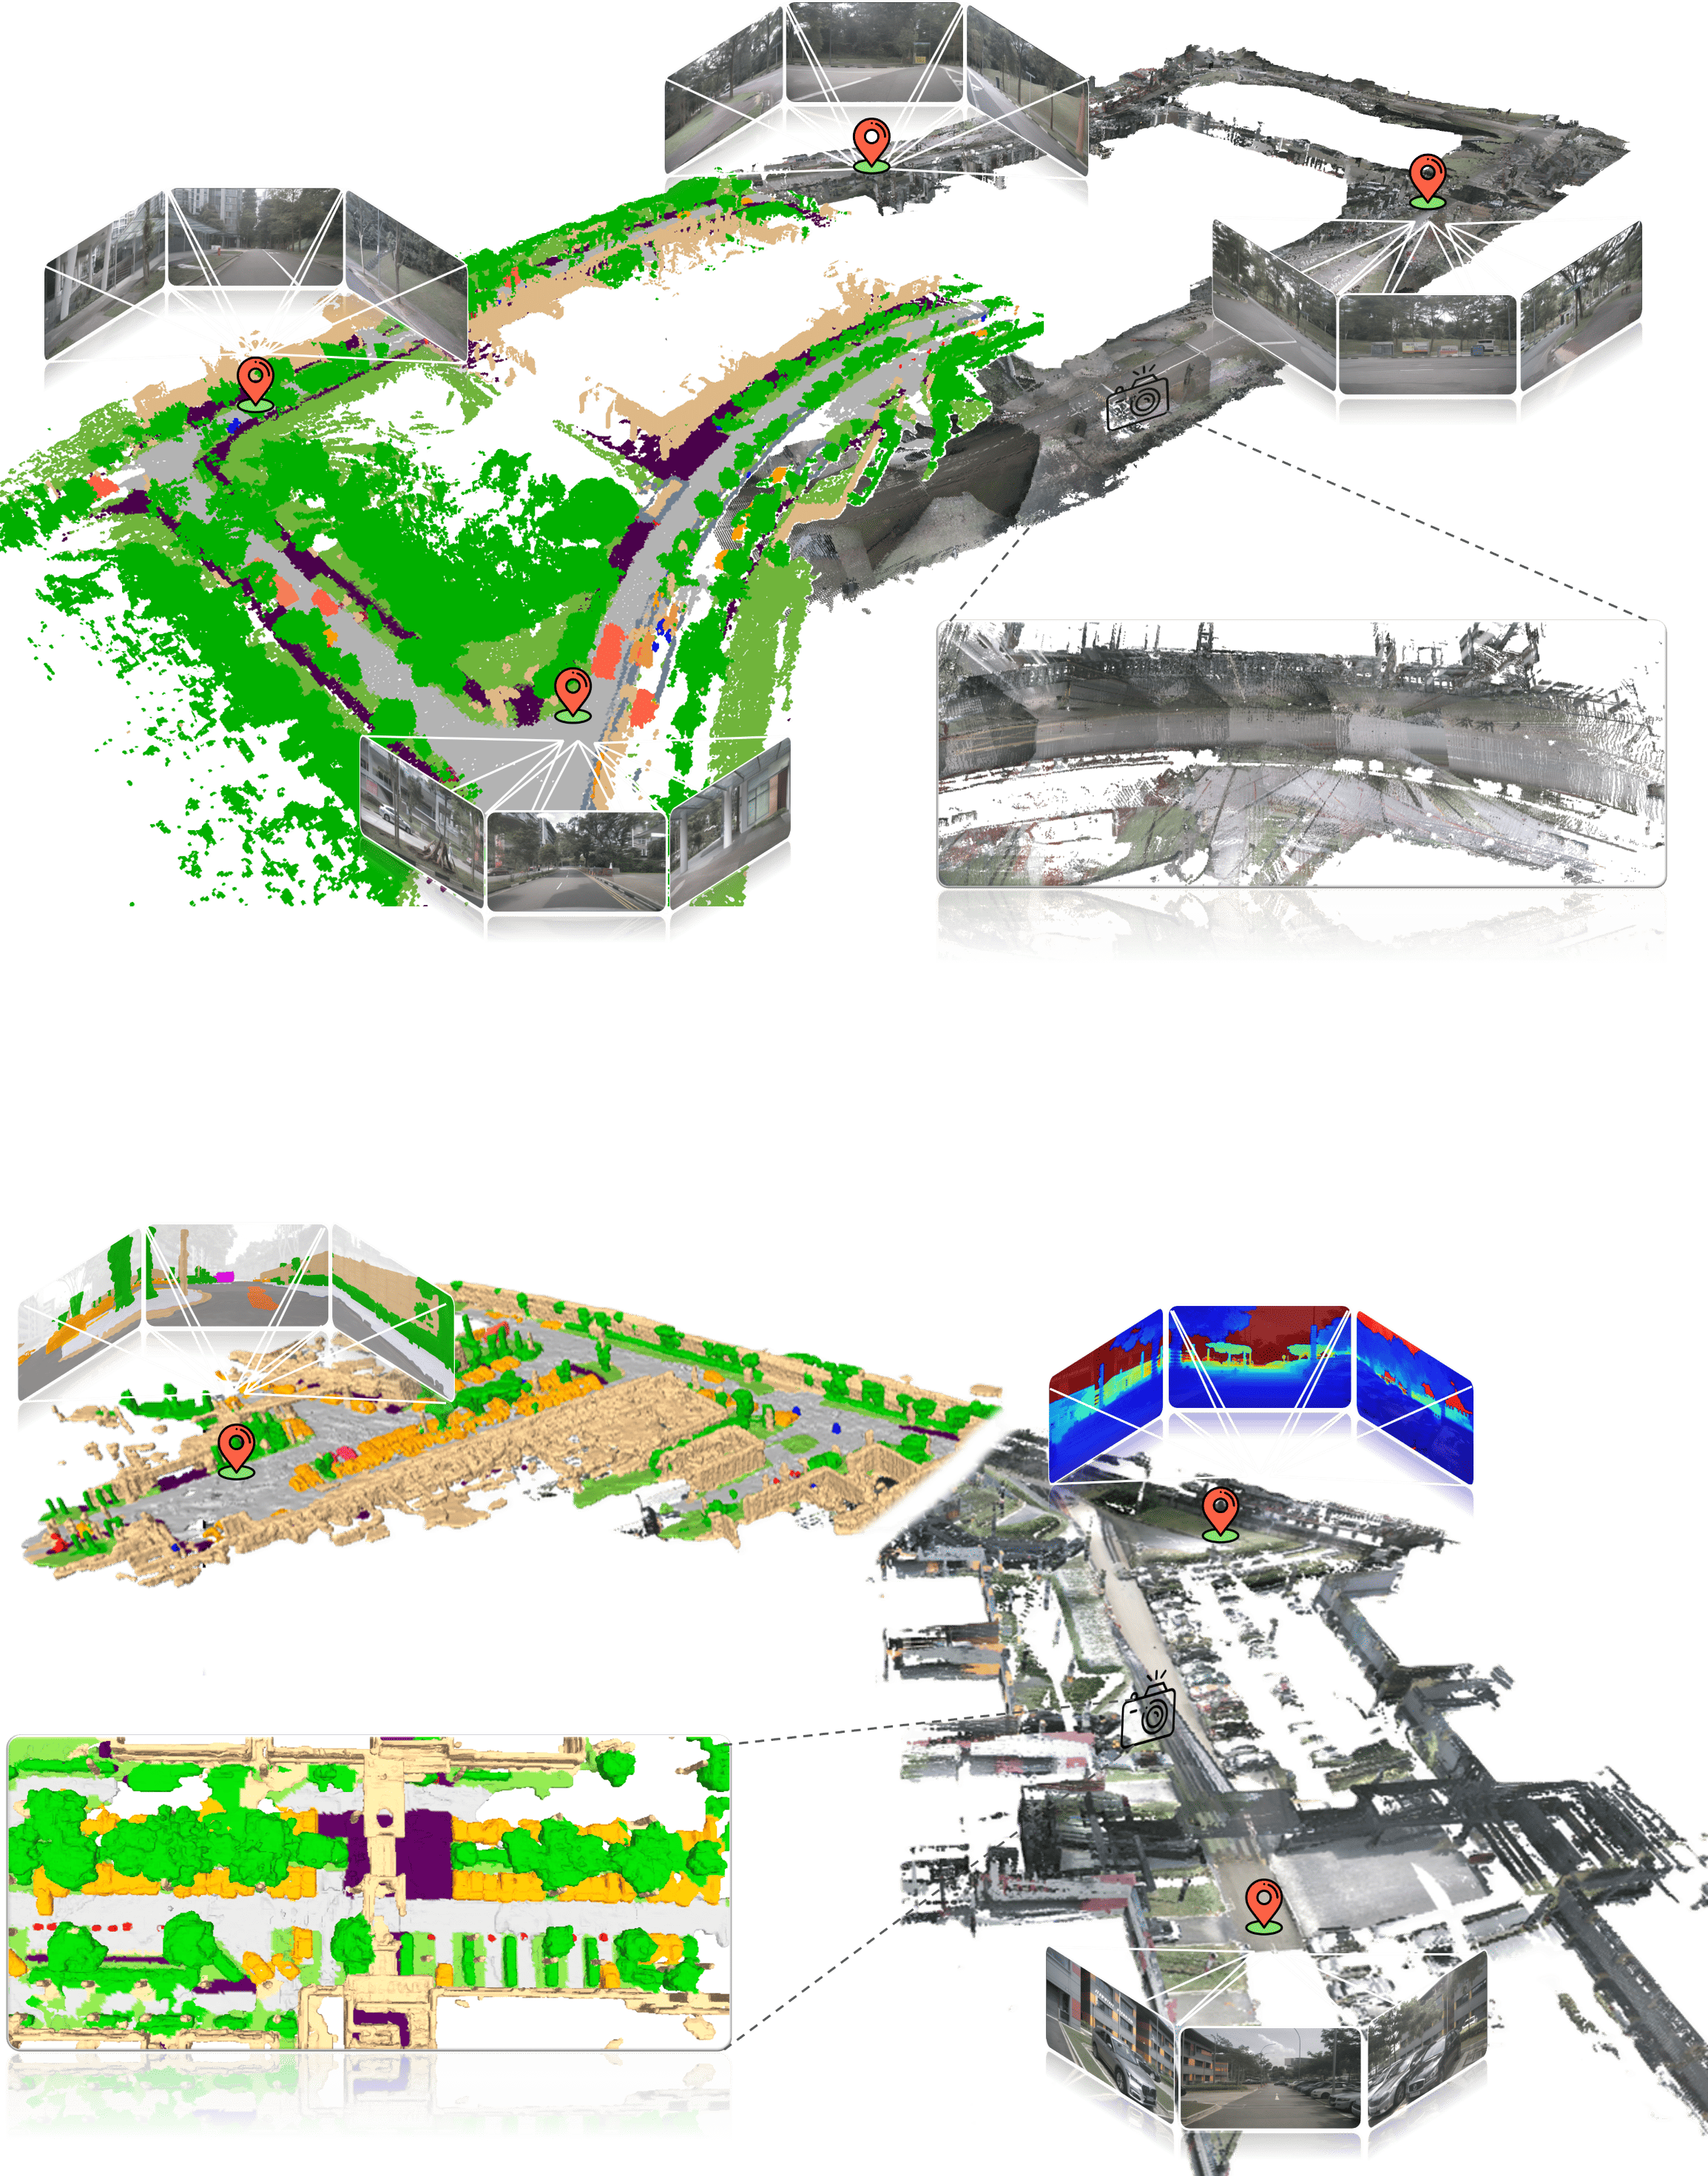
\includegraphics[width=1.0\textwidth]{src/vis_largescale_supp.png}
    % \vspace{-1.5em}
    \caption{\textbf{Qualitative results of large-scale scene generation by {\ours}.} The model extrapolates coherent occupancy fields and multi-view images across extended areas, enabling high-fidelity and complete 3D scene reconstruction. The generated scenes support novel view synthesis of RGB, depth, and occupancy, demonstrating both geometric consistency and high photorealistic quality at scale.}
\label{fig:vis_largescale_supp}
% \vspace{-1mm}
\end{figure}





\clearpage
\subsection{Text-to-Scene Generation}
Figure~\ref{fig:vis_text2scene_1} and Figure~\ref{fig:vis_text2scene_2} illustrate examples of the text-to-scene generation pipeline, which primarily consists of four steps:
\begin{itemize}
[align=right,itemindent=0em,labelsep=2pt,labelwidth=1em,leftmargin=*,itemsep=0em] 
\item Textual scene description generation: Given a coarse user text prompt, the LLM leverages RAG to retrieve semantically relevant scene descriptions from the memory bank, then composes a plausible scene description encompassing scene style, foreground and background elements, and a textual scene-graph layout.
\item Scene-graph to layout generation: The layout diffusion model uses the textual scene-graph to generate the corresponding layout, including object bounding boxes and lane lines.
\item Joint occupancy and multi-view image generation: The occupancy and image diffusion models leverage the layout for geometry control and the text description for semantic control, generating a coherent and realistic 3D occupancy field and multi-view images.
\item Geometry and visual reconstruction: Given the generated voxels and images, we reconstruct the 3D scene while preserving intricate geometry and realistic appearance, supporting various downstream applications.
\end{itemize}

These results demonstrate that the proposed text-to-scene pipeline is an effective and flexible method for driving scene generation.

\subsection{Large-Scale Scene Generation}
Figure~\ref{fig:vis_largescale_supp} illustrates the results of large-scale scene generation. The results show that our method can generate coherent, large-scale driving scenes through consistency-aware extrapolation. Moreover, the generated occupancy and images are fused and lifted for large-scale scene reconstruction, preserving both intricate geometry and realistic visual appearance. The reconstructed scenes support novel RGB, depth, and occupancy rendering.

\section{Potential Societal Impact \& Limitations}
In this section, we discuss the potential societal impact of our work and outline its possible limitations.

\subsection{Societal Impact}
Our proposed framework, {\ours}, for large-scale controllable driving scene generation holds significant potential for real-world societal impact. By unifying fine-grained geometric accuracy with photorealistic visual fidelity, {\method} enables the generation of highly realistic and semantically consistent 3D driving environments. This capability directly supports the development of safer and more efficient autonomous driving systems by enabling rigorous simulation and validation across richly diverse scenarios, including rare cases such as complex intersections, unexpected pedestrian behavior, and unusual road layouts. As a result, {\method} can accelerate the development cycle of autonomous vehicles, reduce reliance on costly and time-consuming real-world data collection, and improve safety standards, ultimately contributing to a reduction in traffic-related accidents and fatalities.

\subsection{Known Limitations}
While {\ours} offers a promising framework for large-scale controllable 3D scene generation, several limitations remain and warrant further investigation.

First, while {\method} supports dynamic 4D scene generation, the current autoregressive video diffusion framework is still limited in long-horizon synthesis. As the number of autoregressive iterations increases, errors in geometry and appearance may accumulate, leading to temporal drift and degraded motion consistency. Future work will focus on improving long-term temporal stability and mitigating error accumulation to achieve more robust and extended video generation.

Second, the scene description memory bank is currently built from the nuScenes dataset~\cite{nuScenes}. While this dataset provides a solid foundation, its limited geometric and semantic diversity may restrict the range and realism of generated scenes. Incorporating additional datasets featuring a broader range of environments, weather conditions, and traffic patterns would enhance the system’s generalization and scene richness.

Third, the occupancy generation pipeline depends on a fixed set of semantic categories predefined in the training data. As a result, introducing new object types or unseen classes requires retraining the model. This rigidity hinders adaptability in evolving or open-world settings. Future work could explore more extensible architectures that support incremental learning or open-vocabulary generation.

Addressing these limitations is essential for enhancing the realism, scalability, and applicability of {\method} in real-world simulation and data generation tasks.

\section{Public Resources Used}
In this section, we acknowledge the public resources used, during the course of this work.

\subsection{Public Datasets Used}
\begin{itemize}
    \item nuScenes\footnote{\url{https://www.nuscenes.org/nuscenes}} \dotfill CC BY-NC-SA 4.0
    
    \item nuScenes-devkit\footnote{\url{https://github.com/nutonomy/nuscenes-devkit}} \dotfill Apache License 2.0

    \item Occ3D\footnote{\url{https://tsinghua-mars-lab.github.io/Occ3D}} \dotfill MIT License
\end{itemize}


\subsection{Public Implementations Used}
\begin{itemize}
    \item MagicDrive\footnote{\url{https://github.com/cure-lab/MagicDrive}} \dotfill Apache License 2.0
    
    \item SemCity\footnote{\url{https://github.com/zoomin-lee/SemCity}} \dotfill MIT License

    \item DynamicCity\footnote{\url{https://github.com/3DTopia/DynamicCity}} \dotfill Unknown

    \item DriveArena\footnote{\url{https://github.com/PJLab-ADG/DriveArena}} \dotfill Apache License 2.0

    \item OccSora\footnote{\url{https://github.com/wzzheng/OccSora}} \dotfill Apache License 2.0

    \item X-Drive\footnote{\url{https://github.com/yichen928/X-Drive}} \dotfill Apache License 2.0

    \item MinkowskiEngine\footnote{\url{https://github.com/NVIDIA/MinkowskiEngine}} \dotfill MIT License

    \item Torch-Fidelity\footnote{\url{https://github.com/toshas/torch-fidelity}} \dotfill Apache License 2.0

    \item Qwen2.5-VL\footnote{\url{https://github.com/QwenLM/Qwen2.5-VL}} \dotfill Apache License 2.0

    \item UniScene\footnote{\url{https://github.com/Arlo0o/UniScene-Unified-Occupancy-centric-Driving-Scene-Generation}} \dotfill Apache License 2.0
\end{itemize}